\documentclass[11pt]{article}
\usepackage{geometry}                % See geometry.pdf to learn the layout options. There are lots.
\usepackage{graphicx}
\usepackage{epstopdf}
\usepackage{amssymb,amsmath}
\usepackage[charter]{mathdesign}
\usepackage{multirow}
\DeclareGraphicsRule{.tif}{png}{.png}{`convert #1 `dirname #1`/`basename #1 .tif`.png}

\textwidth6.5in
\textheight9.0in
\topmargin-0.5in
\oddsidemargin0in
\evensidemargin0in

\title{Material Models Used in NairnMPM and NairnFEA}
\author{John Nairn}
\date{\today} 

\font\tenbsf=cmssbx10 at 11pt
\font\bfsym=cmmib10 at 11pt

\renewcommand{\vec}[1]{\boldsymbol{#1}}
\newcommand{\tens}[1]{\boldsymbol{\mathsf{#1}}}

% definitions
%\def\C{{\fam=9 C}}
\def\A{\hbox{\tenbsf A}}
\def\a#1{\alpha_{#1}}  
\def\B{\hbox{\tenbsf B}}
\def\b#1{\beta_{#1}}  
\def\C{\hbox{\tenbsf C}}
\def\D{\hbox{\tenbsf D}}
\def\dev{\hbox{\tenbsf s}}
\def\ndev{\hbox{\tenbsf n}}
\def\cex{\vec{c}_{excess}}
\def\code#1{{\small\tt #1}}
\def\del{d \vec{\varepsilon}_{e}}
\def\dpl{d \vec{\varepsilon}_{p}}
\def\deff{d \vec{\varepsilon}_{tot}}
\def\df{d \vec{f}}
\def\dfa{d \vec{f}^\alpha}
\def\dfq{d \vec{f}^q}
\def\da{d\vec{\alpha}}
\def\dfW{{\partial f\over \partial W_p}}
\def\dsig{d \vec{\sigma}}
\def\DT{\Delta T}
\def\dq{d\vec q}
\def\dWp{dW_p}
\def\e#1{\varepsilon_{#1}}
\def\ee{\varepsilon}
\def\er#1{\varepsilon_{#1}^{(res)}}
\def\err#1{\varepsilon_{#1}^{(res,r)}}
\def\f{\hbox{\tenbsf f}}
\def\F{\hbox{\tenbsf F}}
\def\fvvec#1#2#3#4#5#6{\left(\begin{array}{ccc} #1 \\ #2 \\ #3 \\ #4 \\ #5 \\ #6 \end{array}\right)}
\def\g#1{\gamma_{#1}}  
\def\I{\hbox{\tenbsf I}}
\def\P{\hbox{\tenbsf P}}
\def\Q{\hbox{\tenbsf Q}}
\def\R{\hbox{\tenbsf R}}
\def\s#1{\sigma_{#1}}  
\def\symmat#1#2#3#4#5#6{\left(\begin{array}{ccc} #1 & #2 & #3 \\ #2 & #4 & #5 \\
                                                      #3 & #5 & #6 \end{array}\right)}
\def\t#1{\tau_{#1}}  
\def\v#1{\nu_{#1}}  
\def\vvec#1#2#3{\left(\begin{array}{ccc} #1 \\ #2 \\ #3 \end{array}\right)}
\def\w#1{\omega_{#1}}  

\begin{document}
\maketitle

\section{Introduction}

These technical notes give details behind the constitutive laws in the material classes implemented in NairnMPM and NairnFEA.

\section{Linear Elastic Materials}

The \code{Isotropic}, \code{TransIsotropic}, and \code{Orthotropic} classes all inherit from the \code{Elastic} class and implement linear elastic materials. The constitutive law is in the \code{Elastic} class and implemented for an orthotropic material. The isotropic and transversely isotropic materials are special cases of the orthotropic material. For such a material, the 3D stiffness equation is
\begin{equation}
     \left(\begin{array}{c} \s{xx} \\ \s{yy} \\ \s{zz} \\ \t{xz} \\ \t{yz} \\ \t{xy} \end{array}\right)
       =  \left(\begin{array}{cccccc}
      C_{11} & C_{12} & C_{13} & 0 & 0 & 0 \\
      C_{12} & C_{22} & C_{23} & 0 & 0 & 0 \\
      C_{13} & C_{23} & C_{33} & 0 & 0 & 0 \\
      0 & 0 & 0 & C_{44} & 0 & 0 \\
      0 & 0 & 0 & 0 & C_{55} & 0  \\
      0 & 0 & 0 & 0 & 0 &  C_{66}  \end{array}\right)
     \left(\begin{array}{c} \e{xx} -\er{xx} \\ \e{yy} -\er{yy} \\ \e{zz} -\er{zz}\\ 
                   \g{xz} \\ \g{yz} \\ \g{xy} \end{array}\right)
\end{equation}
The elements of the $\C$ matrix can be found from all engineering properties. Where $\er{ii}$ are  residual strains in the normal directions. Here they may be caused by either thermal expansion or moisture expansion:
\begin{equation}
\left(\begin{array}{c} \er{xx} \\ \er{yy} \\ \er{zz} \end{array}\right)
       =  \left(\begin{array}{c}
	\a{xx}\DT + \b{xx}\Delta c \\
	\a{yy}\DT + \b{yy}\Delta c \\
	\a{zz}\DT + \b{zz}\Delta c  \end{array}\right)
\end{equation}
where $\a{ii}$ and $\b{ii}$ are thermal and moisture expansion coefficients, and $\DT$ and $\Delta c$ are temperature and moisture change from reference conditions. FEA has only thermal expansion while MPM may have both thermal and moisture expansion.

\subsection{Plane Stress Equations}

The plane stress stiffness equations for in-plane stresses are
\begin{equation}
      \vvec{\s{xx}}{\s{yy}}{\t{xy}} = \symmat{Q_{xx}}{Q_{xy}}{0}{Q_{yy}}{0}{Q_{xyxy}}
          \vvec{\e{xx} - \er{xx}}{\e{yy} - \er{yy}}{\g{xy}}
 \end{equation}
The elements of the $\Q$ matrix are found from
\begin{eqnarray}%
   Q_{xx} &  = &  {E_{xx}\over 1 - \v{xy}\v{yx}} \\
   Q_{yy} & = & {E_{yy}\over 1 - \v{xy}\v{yx}} \\
   Q_{xy} &  = & {E_{xx}\v{yx}\over 1 - \v{xy}\v{yx}}  =  {E_{yy}\v{xy}\over 1 - \v{xy}\v{yx}}\\
   Q_{xyxy} & = &  G_{xy} 
\end{eqnarray}%
These elements are calculated in \code{SetAnalysisProps()} as \code{C11} = $Q_{xx}$, \code{C12} = $Q_{xy}$, \code{C22} = $Q_{yy}$, and \code{C66} = $Q_{xyxy}$. The thermal  and moisture expansion coefficients are equal to the material thermal  and moisture expansion coefficients and set as \code{CTE1} $=\a{xx}$, \code{CTE2} $=\a{yy}$, \code{CME1} $=\b{xx}$, and \code{CME2} $=\b{yy}$, also in \code{SetAnalysisProps()}.

In plane stress analysis, $\s{zz}=0$, but $\e{zz}\ne0$. The out-of-plane strain is found from the 3D stiffness matrix by solving the $\s{zz}$ equation for $\e{zz}$:
\begin{equation}
            \e{zz} = -{C_{13}\over C_{33}}(\e{xx} -\a{xx}\DT) - {C_{23}\over C_{33}}(\e{yy} -\a{yy}\DT) 
                     + \er{zz}
\end{equation}
The new terms are set in \code{SetAnalysisProps()} as \code{C13} $=-C_{13}/C_{33}$, \code{C23} $=-C_{23}/C_{33}$, \code{CTE3} $=\a{zz}$, and \code{CME3} $=\b{zz}$.

\subsection{Plane Strain Equations}

The plane strain stiffness equations for in-plane stresses are
\begin{equation}
      \vvec{\s{xx}}{\s{yy}}{\t{xy}} = \symmat{C_{11}}{C_{12}}{0}{C_{22}}{0}{C_{66}}
          \vvec{\e{xx} -\err{xx}}{\e{yy} - \err{yy}}{\g{xy}}
 \end{equation}
 where residual strains now depend on reduced residual strains
\begin{equation}
\left(\begin{array}{c} \err{xx} \\ \err{yy}  \end{array}\right)
       =  \left(\begin{array}{c}
	 \er{xx} + \v{zx}\er{zz} \\
	\er{yy} + \v{zy}\er{zz} \end{array}\right)
\end{equation}
which is equivalent to using reduced expansion properties
\begin{equation}
\left(\begin{array}{c} \err{xx} \\ \err{yy}  \end{array}\right)
       =  \left(\begin{array}{c}
	 \a{xx}^{(r)}\DT + \b{xx}^{(r)}\Delta c \\
	\a{yy}^{(r)}\DT + \b{xx}^{(r)}\Delta c \end{array}\right)
\end{equation}
The reduced expansion coefficients are
\begin{eqnarray}%
   \a{xx}^{(r)} = \a{xx} + \v{zx}\a{zz}, \ \ 
   \a{yy}^{(r)} = \a{yy} + \v{zy}\a{zz}, \ \ 
   \b{xx}^{(r)} = \b{xx} + \v{zx}\b{zz}, \ \ 
   \b{yy}^{(r)} = \b{yy} + \v{zy}\b{zz}
\end{eqnarray}%
These elements are calculated in \code{SetAnalysisProps()} as \code{C11} $=C_{11}$, \code{C12}  $=C_{12}$, \code{C22} $=C_{22}$, and \code{C66} $=C_{66}$. The reduced expansion coefficients are set as \code{CTE1} $=\a{xx}^{(r)}$, \code{CTE2} $=\a{yy}^{(r)}$, \code{CME1} $=\b{xx}^{(r)}$, and \code{CME2} $=\b{yy}^{(r)}$, also in \code{SetAnalysisProps()}.

In plane strain analysis, $\e{zz}=0$, but $\s{zz}\ne0$. The out-of-plane stress is found from the 3D stiffness matrix by setting $\e{zz}=0$:
\begin{eqnarray}
            \s{zz} & = & C_{13}\bigl(\e{xx} -(\a{xx}^{(r)}-\v{zx}\a{zz})\DT - (\b{xx}^{(r)}-\v{zx}\b{zz})\Delta c\bigr)
 \nonumber\\
 &&\qquad\mbox{}
                     +C_{23}\bigl(\e{yy} -(\a{yy}^{(r)}-\v{zy}\a{zz})\DT-(\b{yy}^{(r)}-\v{zy}\b{zz})\Delta c\bigr) 
                     -C_{33} \er{zz}
\end{eqnarray}
The new terms are set in \code{SetAnalysisProps()} as \code{C13} $=C_{13}$, \code{C23} $=C_{23}$, and \code{C33} $=C_{33}$. Notice that this equation needs actual residual expansion coefficients and thus the reduced expansion coefficients must be {\em unreduced} by subtracting terms. For these calculations (more details in next section), the following expansion properties are set as \code{CTE3} $=\a{zz}$, \code{CME3} $=\b{zz}$, \code{prop1} $=\v{zx}$, and \code{prop2} $=\v{zy}$.

\subsection{Rotated Stiffness Equations in MPM}

For orthotropic materials with material angle not zero, the stiffness equations must be rotated counter-clockwise by the material point angle to transpose to the analysis coordinate systems. The material point angle is initialized when the calculations starts. To account for large displacements and rotations, the angle is updated on each time step based on the rotation tensor. The angle thus always reflects the current material orientation. Thus prior to calling \code{MPMConstitutiveLaw()}, the equations are rotated (if needed) to obtain:
\begin{equation}
      \vvec{\s{xx}}{\s{yy}}{\t{xy}} = \symmat{\code{C[1][1]}}{\code{C[1][2]}}
                      {\code{C[1][3]}}{\code{C[2][2]}}{\code{C[2][3]}}{\code{C[3][3]}}
          \vvec{\e{xx} - \er{xx}}{\e{yy} - \er{yy}}{\g{xx}-\er{xy}}
 \end{equation}
 where the rotated residual strains (which become reduced residual strains when in plane strain) are
\begin{equation}
\left(\begin{array}{c} \er{xx} \\ \er{yy} \\ \er{xy} \end{array}\right)
       =  \left(\begin{array}{c}
	\code{alpha[1]}\DT + \code{beta[1]}\Delta c \\
	\code{alpha[2]}\DT + \code{beta[2]}\Delta c \\
	\code{alpha[3]}\DT + \code{beta[3]}\Delta c  \end{array}\right)
\end{equation}
 The rotated elements are found by standard in-plane rotation in the counter-clockwise direction in \code{LoadMechanicalPropertiesFEA()}. Rotation is only needed for anistotropic materials. For isotropic materials, the \code{C[][]}, \code{alpha[]}, and \code{beta[]} elements are calculated once for zero rotation angle. The elements of \code{C[][]} are also made specific by dividing by material density. The constitutive law should only use specific properties to have the proper specific stress.
 
Calculation of out-of-plane values requires rotation of the 3D stiffness matrix counter-clockwise around the $z$ axis. The results for plane stress are
\begin{eqnarray}
     \e{zz} & = & \code{C[4][1]} (\e{xx} - \er{xx}) +  \code{C[4][2]}(\e{yy} -\er{yy}) 
     \nonumber \\
     && \qquad\qquad\mbox{}
                 + \code{C[4][3]}(\g{xy}-\er{xy})  + \er{zz}
\end{eqnarray}
where 
\begin{eqnarray}
 \code{C[4][1]} & = &-\left({C_{13}\over C_{33}}\cos^2\theta + {C_{23}\over C_{33}}\sin^2\theta\right)
        = \code{C13}\cos^2\theta + \code{C23}\sin^2\theta  \\
 \code{C[4][2]} & = &-\left({C_{13}\over C_{33}}\sin^2\theta + {C_{23}\over C_{33}}\cos^2\theta\right)
        = \code{C13}\sin^2\theta + \code{C23}\cos^2\theta  \\
 \code{C[4][3]} & = &  \left({C_{13}\over C_{33}} - {C_{23}\over C_{33}}\right)\sin\theta\cos\theta
        = -(\code{C13}-\code{C23})\sin\theta\cos\theta
\end{eqnarray}
and \code{CTE3} = \code{alpha[4]} $=\a{zz}$ and \code{CME3} = \code{beta[4]} $=\b{zz}$ hold out-of-plane thermal expansion coefficients needed to find $\er{zz}$, which was defined earlier.

The problem in plane strain is that the calculation of $\s{zz}$ requires rotated expansion coefficients while the \code{alpha[1]} to \code{alpha[3]}  and \code{beta[1]} to \code{beta[3]} have rotated {\em reduced\/} expansion coefficients. The solution is to define some new terms such that
\begin{eqnarray}
     \s{zz} & = & \code{C[4][1]} (\e{xx} -(\err{xx}-\code{alpha[5]}\er{zz}))
                         +  \code{C[4][2]}(\e{yy} -(\err{yy}-\code{alpha[6]}\er{zz})) 
     \nonumber \\
     && \qquad\qquad\mbox{}
                 + \code{C[4][3]}(\g{xx}-(\err{xy}-\code{alpha[7]}\er{zz}))  - \code{C[4][4]} \er{zz}
\end{eqnarray}
where
\begin{eqnarray}
 \rho\thinspace \code{C[4][1]} & = &C_{13}\cos^2\theta + C_{23}\sin^2\theta
            = \code{C13}\cos^2\theta + \code{C23}\sin^2\theta  \\
 \rho\thinspace \code{C[4][2]} & = &C_{13}\sin^2\theta + C_{23}\cos^2\theta
             = \code{C13}\sin^2\theta + \code{C23}\cos^2\theta  \\
 \rho\thinspace \code{C[4][3]} & = & - \left(C_{13} - C_{23}\right)\sin\theta\cos\theta
             =  -(\code{C13}-\code{C23})\sin\theta\cos\theta \\
 \rho\thinspace \code{C[4][4]} & = & C_{33}  \\
  \code{alpha[5]} & = &\v{zx}\cos^2\theta + \v{zy}\sin^2\theta
         = \code{prop1}\cos^2\theta + \code{prop2}\sin^2\theta  \\
  \code{alpha[6]} & = &\v{zx}\sin^2\theta + \v{zy}\cos^2\theta
        = \code{prop1}\sin^2\theta + \code{prop2}\cos^2\theta  \\
  \code{alpha[7]} & = & - 2\left(\v{zx} - \v{zy}\right)\sin\theta\cos\theta 
       =  -2(\code{prop1}-\code{prop2})\sin\theta\cos\theta
\end{eqnarray}
Again, \code{CTE3} = \code{alpha[4]} $=\a{zz}$ and \code{CME3} = \code{beta[4]} $=\b{zz}$ hold out-of-plane expansion coefficients needed to find $\er{zz}$, which was defined earlier.
In these terms, $\err{xx}-\code{alpha[5]}\er{zz}$ (and similarly for ($yy$, 6) and ($xy$, 7) pairs) evaluate to the rotated, but {\em unreduced\/} expansion strains. The angle $\theta$ is the material angle on the material point, which is a clockwise rotation from the analysis axes.

\subsection{Rotated Stiffness Equations in FEA}

To be added.

\section{Plasticity Materials}

For general analysis, begin with an elastic stress increment, $\dsig$, given by
\begin{equation}
    \dsig = \C \deff 
\end{equation}
where $\C$ is the stiffness matrix, $\deff=d\vec\varepsilon-d\vec\varepsilon_{res}$ is total strain increment (using tensorial strains) relative to the residual strain increments. Let $f(\vec{\sigma},\vec q)$ be a plastic potential function that depends on components of stress, possibly on some collection of internal variables ($\vec q$) or other parameters. The potential function is defined such that $f=0$ is the yield surface, $f<0$ is the elastic region, and $f>0$ is not allowed.

First construct a trial update that assumes elastic deformation only or assumes that $\del=\deff$, $\dpl=0$, and $d\vec q=0$ (in other words, no plastic deformation). The trial $f$ is given by\begin{equation}
       f_{trial} = f(\vec\sigma + \dsig,\vec q) = f(\vec\sigma + \C \deff ,\vec q)
\end{equation}
If $f_{trial}<0$, the deformation is elastic, the trial increment is accepted, and the analysis is done.

If $f_{trial}>0$, the task is to partition the total strain into elastic and plastic strain, $\deff=\del+\dpl$, such that the final $f$ is zero. In other words, the task is to solve
\begin{equation}
     f(\vec\sigma + \C \deff  - \C\dpl,\vec q + \dq) = 0
\end{equation}
By the associative flow rule, the increment in plastic strain and internal variables are assumed to be 
\begin{equation}
      \dpl = \lambda\df   \qquad {\rm and}\qquad \dq = -\lambda \vec h(\sigma,\vec q)
\end{equation}
where
\begin{equation}
      df_i = {\partial f\over \partial\sigma_i}   
\end{equation}
are the derivatives of $f$ with respect to the components of stress and the internal variables and $\vec h$ is function of stress and internal variable state). Thus, the task is to solve
\begin{equation}
     f(\vec\sigma + \C \deff - \lambda\C\df,\vec q -\lambda \vec h) = 0
\end{equation}
for $\lambda$. For arbitrary $f$, this solution may require numerical analysis.

If all increments are small, and $f$ depends only on stress and internal variables, the problem can be expanded around $f_{trial}$ in a Taylor series to give
\begin{equation}
    f  = f_{trial} - \lambda\Bigl( \df \cdot \C \df + \dfq \cdot \vec h \Bigr)
\end{equation}
where
\begin{equation}
\dfq_i = {\partial f\over \partial q_i}
\end{equation}
Setting the new $f$ to zero to land on the yield surface, this equation can be solved for $\lambda$ and thus solved to partition the strain increment into elastic and plastic strain. The solution is
\begin{equation}
        \lambda = { f_{trial}   \over  \df\cdot \C\df + \dfq \cdot \vec h }     \label{lambdaInitial}
\end{equation}

For larger increments or more accurate solution, the problem can be solved iteratively by Newton's method with bracketing. The following method is only used in the code for anisotropic materials because special case results that seem to work well for isotropic materials are given below. Here is method used for anisotropic materials.

\begin{enumerate}

\item Find an initial guess for $\lambda^{(2)}=\lambda$ from the Eq.~(\ref{lambdaInitial}) where $\df$ and $\vec h$ are found from ${\vec\sigma_{trial}}$ or stress when $\lambda=0$ and $\dfq$ is found from initial $\vec q$.

\item Update stress at initial guess in two steps
\begin{eqnarray}
      {\vec\sigma}^{(1)} & = & {\vec\sigma_{trial}} - \lambda^{(2)}\C\df({\vec\sigma_{trial}}) \\
      {\vec\sigma}^{(2)} & = & {\vec\sigma_{trial}} - \lambda^{(2)}\C\df({\vec\sigma}^{(1)}) 
\end{eqnarray}

\item Find new $\df$ and $\vec h$ using ${\vec\sigma}^{(2)}$ followed by calculation of $f_2$ corresponding to $\lambda_2$:
\begin{equation}
     f^{(2)} =  f({\vec\sigma}^{(2)},\vec q^{(0)} - \lambda^{(2)} \vec h({\vec\sigma}^{(2)}))
\end{equation}

\item Pick a lower $\lambda$ and calculate $f$:
\begin{eqnarray}
     \lambda^{(1)} & = & {\lambda^{(2)}\over 2} \\
      {\vec\sigma}^{(1)} & = & {\vec\sigma_{trial}} - \lambda^{(1)}\C\df({\vec\sigma}^{(2)}) \\
     f^{(1)} & = &  f({\vec\sigma}^{(1)},\vec q^{(0)} - \lambda^{(1)} \vec h({\vec\sigma}^{(2)}))
\end{eqnarray}

\item Expand the interval $\lambda^{(1)}$ to $\lambda^{(2)}$ as needed until it brackets a solution for $f=0$. The code follows {\tt zbrac()} in ``Numerical Recipes in C'' (page 260). Whenever need new value for $f$, use:
\begin{eqnarray}
      {\vec\sigma}^{(k)} & = & {\vec\sigma_{trial}} - \lambda^{(k)}\C\df({\vec\sigma}^{(2)}) \\
     f^{(k)} & = &  f({\vec\sigma}^{(k)},\vec q^{(0)} - \lambda^{(k)} \vec h({\vec\sigma}^{(2)}))
\end{eqnarray}
In other words, use the slopes calculated in step 3 above throughout the calculation. Attempts to recalculate the slope on each step tended to cause problems. If the bracketing fails, return the initial $\lambda$ from step 1 as an approximate result.

\item Solve for $\lambda$ using Newton-Raphson method with derivatives and bracketing following {\tt rtsafe()} in ``Numerical Recipes in C'' (page 273). Whenever needed, find $f$ and its derivative from
\begin{eqnarray}
      {\vec\sigma}^{(k)} & = & {\vec\sigma_{trial}} - \lambda^{(k)}\C\df({\vec\sigma}^{(2)}) \\
      \vec q^{(k)} & = & \vec q^{(0)} - \lambda^{(k)} \vec h({\vec\sigma}^{(2)}) \\
      f^{(k)} & = &  f({\vec\sigma}^{(k)},\vec q^{(k)})  \\
      {df^{(k)}\over d\lambda} & = & -\left( \df({\vec\sigma}^{(2)})\cdot \C\df({\vec\sigma}^{(2)}) + \dfq(\alpha^{(k)}) \cdot \vec h({\vec\sigma}^{(2)})\right) 
\end{eqnarray}
Again, the key slopes are found from the initial stress guess in ${\vec\sigma}^{(2)}$. Attempts to update slopes as solution proceeds were less stable and also slower. It might be possible to update slopes after solution, re-bracket the solution and repeat, but it may not improve accuracy much.

\item Continue until convergence.

\end{enumerate}

\subsection{$J_2$ Flow Theory for Isotropic Materials}

For a special case, consider an isotropic material with isotropic hardening, a single internal variable, $\alpha$, and assume the plastic potential is a function only of $J_2= (1/2)\|\dev\|^2$ expressed as
\begin{equation}
      f = \|\dev\| - \sqrt{2\over3} K(\alpha) = \|\dev\| - \sqrt{2\over3}(\sigma_y - q)
\end{equation}
where $\dev$ is the deviatoric stress tensor and $K(\alpha)$ defines the tensile yield stress as a function of the hardening variable and possibly other variables ({\it e.g.}, plastic strain rate or temperature, but not pressure). The plastic variable $q$ and $\alpha$ are related by
\begin{equation}
      q  = \sigma_y - K(\alpha)
\end{equation}
The usual assumption is to take
\begin{equation}
        d\alpha = \lambda\sqrt{2\over3}  \quad{\rm which\ implies} 
        \quad dq = -\lambda K'(\alpha)\sqrt{2\over3}  \quad{\rm and} 
        \quad h = K'(\alpha)\sqrt{2\over3}
\end{equation}
All materials that fit this mold are handled in {\tt NairnMPM} by the {\tt IsoPlasticity} class. The implementation of hardening law ($K(\alpha)$) is handled by a separate subclass of the {\tt HardeningLawBase} class. Combining {\tt IsoPlasticity} class with various hardening laws gives a series of material. The only materials that need to subclass {\tt IsoPlasticity} is if they need a different equation of state to handle elastic parts differently.

In terms of the deviatoric stress
\begin{equation}
     2J_2 = \|\dev\|^2 =  s_{xx}^2 + s_{yy}^2  + s_{zz}^2 + 2s_{xy}^2 + 2s_{xz}^2 + 2s_{yz}^2 \\
 \end{equation}
During plastic deformation, 
the plastic strain increment simplifies to
\begin{equation}
     \lambda \df = \lambda {\dev_{trial}\over \|\dev_{trial}\|} = \lambda \ndev
\end{equation}
where $ \dev_{trial}$ is the deviatoric stress calculated by assuming no plastic deformation.
Since $\|\dpl\| = \|\lambda \df\| = \lambda$, this assumption corresponds to
\begin{equation}
     d\alpha = \sqrt{2\over3}\thinspace \|\dpl\|
\end{equation}
where $\sqrt{2\over3}\|\dpl\|$ is known as the equivalent plastic strain increment. In other words, $\alpha$ is the cumulative equivalent plastic strain. During uniaxial plastic deformation, the equivalent plastic strain will equal the axial plastic strain ({\em i.e.} when $d\varepsilon_{xx}=d\varepsilon$ and $d\varepsilon_{yy}=d\varepsilon_{zz} = -d\varepsilon/2$, $\sqrt{2\over3}\|\dpl\| = d\varepsilon$).

Once $\lambda$ is known, the final deviatoric stress is written as
\begin{equation}
        \dev = \dev_{trial} - \lambda 2G\ndev = \left(1- {\lambda 2G\over \|\dev_{trial}\|}\right) \dev_{trial}
\end{equation}
which leads to
\begin{equation}
         \|\dev\| =  \|\dev_{trial}\| - \lambda 2G \qquad {\rm and} \qquad 
         {\dev\over \|\dev\|} = {\dev_{trial}\over \|\dev_{trial}\|}
\end{equation}
The required equation for finding $\lambda$ thus simplifies to depend only on $\|\dev_{trial}\|$, $G$, and hardening law:
\begin{equation}
      f^{(k)} = \|\dev\| -  \sqrt{2\over3} K(\alpha^{(k)}) = \|\dev_{trial}\| - \lambda^{(k)} 2G -  \sqrt{2\over3} K(\alpha^{(k)}) = 0
\end{equation}
This can be solved in the iterative method above with the specific results of:
\begin{eqnarray}
        {df^{(k)}\over d\lambda} & = & -2G - \sqrt{2\over3}{dK(\alpha^{(k)})\over d\lambda}  = -2G - {2K'(\alpha^{(k)})\over 3} \\
        \alpha^{(k+1)} & = & \alpha^{0} +  \lambda^{(k+1)} \sqrt{2\over3}
\end{eqnarray}
where $K'(\alpha^{(k)})$ is the derivative with respect to $\alpha$. This solution is implemented by hardening law classes. The {\tt HardeningLawBase} class solves this equation numerically by having a subclass providing for calculation of $K(\alpha^{(k)})$ (in \code{GetYield()}) and $\sqrt{2\over3}{dK(\alpha^{(k)})\over d\lambda}$ (in \code{GetKPrime()}). The base class uses Newton's method with bracketing; the bracketing is needed because some yield functions are unstable by the unbracketed Newton's method. The solution is done in {\tt SolveForLambdaBracketed()} as follows:

\begin{enumerate}

\item The result for $\lambda=0$ is known to have $f>0$.

\item Set the plastic strain rate $d\alpha/dt$ to 1 sec$^{-1}$ where $dt$ is time step and then trial $\lambda=d\alpha/\sqrt{2/3}$.

\item Evaluate $f$; if it is negative, $\lambda$ is between current value and previous order of magnitude; if it is positive, increase the strain rate by a factor or 10 and go back to beginning of this step.

\end{enumerate}

If any subclass hardening law can bracket the solution faster (or find the solution with an unbracketed method), it can override {\tt SolveForLambdaBracketed()} and provide a new method (which may be as simple as calling the unbracketed method in {\tt SolveForLambda()} or devising a better bracketing method in {\tt BracketSolution()}). For example, for a linear hardening law, $\lambda$ can be found in a closed-form expression --- when $K(\alpha)=\sigma_Y + E_p\alpha$, the task is to solve
\begin{equation}
      f =  \|\dev_{trial}\| - \lambda 2G -  \sqrt{2\over3} \left(\sigma_Y + E_p\left(\alpha^{0}+ \lambda \sqrt{2\over3}\right)\right) = 0
\end{equation}
The analytical solution is
\begin{equation}
      \lambda = { \|\dev_{trial}\| - \sqrt{2\over3}\left(\sigma_Y + E_p\alpha^{0} \right) \over  2G +  {2E_p\over3} }
\end{equation}

\subsection{Plane Strain and Axisymmetric Analysis for $J_2$ Flow Theory, Isotropic Materials}

Plane strain and axisymmetric analysis can follow the above analysis. For isotropic material models, it is convenient to formulate in terms of bulk and shear moduli ($K$ and $G$) and track pressure and deviatoric stress. The stress update is
\begin{eqnarray}
       {\Delta V\over V} & = & d\varepsilon_{xx} + d\varepsilon_{yy} + d\varepsilon_{zz}  - 3d\er{} \\
       dP & = & -K {\Delta V\over V} \\
       ds_{ij}^{trial} & = & 2G \left(d\varepsilon_{ij}^{(tot)} - {\Delta V\over 3V}\right)   \qquad {\rm for\ }i=j=x,y,z\\
       d\tau_{xy} = ds_{xy} & = & G d\gamma_{xy} \\
\end{eqnarray}
where
\begin{equation}
      d\varepsilon_{xx}^{(tot)} = d\varepsilon_{xx} - d\er{}, \quad
      d\varepsilon_{yy}^{(tot)} = d\varepsilon_{yy} - d\er{}, \quad {\rm and}\quad
      d\varepsilon_{zz}^{(tot)} =  d\varepsilon_{zz} - d\er{}
\end{equation}
are the strain increments relative to the increment in residual strain (note that in plane strain, $ d\varepsilon_{zz}=0$, but it may be nonzero when axisymmetric). For isotropic materials, only normal residual strains exist and they are all equal to
\begin{equation}
      d\er{} = \a{}\DT + \b{}\Delta c
\end{equation}
If the updated stress has $f<0$, the analysis uses the new stress state.

If $f>0$, the equations in the previous section are used to find $\lambda$. Once $\lambda$ is known, the initial update is modified using
\begin{equation}
     ds_{ij} = ds_{ij}^{trial} - 2G d\varepsilon_{ij}^{p} 
\end{equation}
while the pressure update is unchanged.
By including $\s{zz}$ in the calculations, the out-of-plane stress is correctly updated. In general, the plastic strain will include plastic strain in the $z$ direction, even in plane strain. To keep zero total strain when in plane strain analysis, the out-of-plane elastic strain update will be
\begin{equation}
       d\varepsilon_{ij}^{e} = -d\varepsilon_{ij}^{p}  
\end{equation}

For the \code{IsoPlasticity} class, $K=$ \code{Kred}, $G=$ \code{Gred}, $\a{}=$ \code{CTE3}, and $\b{}=$ \code{CME3}. The default implementation assumes these are constant and they are calculated once in \code{VeriofyAndLoadProperties()}. A subclass can implement non-linear materials two ways. To let $K$, $G$, $\a{}$, and $\b{}$, depend on particle state, calculate their state-dependent values in \code{LoadMechanicalProps()} and/or \code{GetTransportProps()}. An alternative approach for more complicated materials is to replace the pressure calculation by overriding \code{UpdatePressure()} . This method is called after finding ${\Delta V/V}$, but before any other calculations. It must update the particle pressure and particle strain energy due to dilation. It should also calculate $G$ (in \code{Gred}) if it depends on particle state. It need not calculate $K$ (in \code{Kred}) because it is not needed after new pressure is found. 

\subsection{Plane Stress Analysis for $J_2$ Flow Theory, Isotropic Materials}

Unfortunately, plane stress analysis requires some addition steps and always requires numerical solution for $\lambda$. First, by requiring $\s{zz}=0$, the 3D equations can be solved to show
\begin{equation}
         d\varepsilon_{zz}^{(tot)} = - {\nu\over 1-\nu}\left(d\varepsilon_{xx}^{(tot)} + d\varepsilon_{yy}^{(tot)}\right)
\end{equation}
Using this relation, the stress update for the in-plane terms only are
\begin{eqnarray}
       {\Delta V\over V} & = & d\varepsilon_{xx}^{(tot)} + d\varepsilon_{yy}^{(tot)} + d\varepsilon_{zz}^{(tot)}
                             = \left(1-2\nu\over 1-\nu\right)\left(d\varepsilon_{xx}^{(tot)} + d\varepsilon_{yy}^{(tot)}\right)      \label{psDelV} \\
       dP & = & -K {\Delta V\over V} \\
       ds_{ij}^{trial} & = & 2G \left(d\varepsilon_{ij}^{(tot)} - {\Delta V\over 3V}\right)   \qquad {\rm for\ }i=j=x,y \\
       ds_{zz}^{trial} = ds_{zz} & = & dP \\
       d\tau_{xy}^{trial} = ds_{xy}^{trial} & = & G d\gamma_{xy} \\
\end{eqnarray}
The \code{IsoPlasticity} class is based on $K$ and $G$ (in \code{Kred} and \code{Gred}). For calculation efficiency, two above terms and one term defined below are stored in variables:
\begin{eqnarray}
       \code{psRed} & = & \left(1-2\nu\over 1-\nu\right) = {1 \over {K\over 2G} + {2\over 3}} \\
       \code{psLr2G} & = & {\nu\over 1-\nu} ={{K\over 2G} - {1\over 3} \over {K\over 2G} + {2\over 3}} \\
       \code{psKred} & = & {E\over 3(1-\nu)} = K*\code{psRed} = {K \over {K\over 2G} + {2\over 3}}
\end{eqnarray}
Note that plane stress analysis assumes incrementally linear-elastic response (although the linear terms can depend on particle state) and also needs to know \code{psRed}  \emph{before} finding the pressure change. Materials that override \code{LoadMechanicaProps()} must calculate \code{psRed}, \code{psLr2G}, and \code{psKred} along with \code{Kred} and \code{Gred}. Materials that override \code{UpdatePressure()} instead will need to deal with these terms differently. For such materials, the incremental volumetric strain passed to \code{UpdatePressure()} depends on \code{psRed} (see Eq.~(\ref{psDelV})). The best approach is to set $\code{psRed}=1$ and then scale \code{delV} by the current $(1-2\nu)/(1-\nu)$ in \code{UpdatePressure()}. That method can leave $\code{psRed}=1$ (because it is no longer needed) and calculate \code{psLr2G} (for normal stress update) and \code{psKred} (for finding $\lambda$) needed in subsequent calculations. It should also calculate \code{Gred}, but \code{Kred} is not needed.

When $f>0$, the process (following Simo and Hughes), effectively (or equivalently) revises $f$ using squares to be
\begin{equation}
       f = \|\dev\|^2 - {2\over 3}K^2(\alpha) = \sigma \P\sigma - {2\over 3}K^2(\alpha)
\end{equation}
where $\P$ is a transformation matrix on the plane stress vector $\sigma = (\s{xx}, \s{yy}, \tau_{xy})$ given by
\begin{equation}
          \P = \left( \begin{array}{rrr}
                    {2\over 3} & -{1\over 3} & 0 \\ 
                    -{1\over 3} & {2\over 3} & 0 \\ 0 & 0 & 2 \end{array}\right)
\end{equation}
such that $\sigma \P\sigma = \|\dev\|^2$. The plastic strain update from this $f$, and using engineering shear strain, is
\begin{equation}
     (d\varepsilon_{xx}^p,  d\varepsilon_{yy}^p, d\gamma_{xy}^p) = \lambda \df = \lambda \P\sigma
\end{equation}
Now, in this flow theory, the total volume change due to plastic strains is zero; thus this plastic strain increment implies $d\varepsilon_{zz}^p = - (d\varepsilon_{xx}^p + d\varepsilon_{yy}^p)$. The full 3D plastic strain increment tensor using tensorial strains is
\begin{equation}
          \dpl = \lambda \left( \begin{array}{ccc}
                    {1\over 3}(2\s{xx}-\s{yy})& \tau_{xy} & 0 \\ 
                    \tau_{xy} & {1\over 3}(2\s{yy}-\s{xx}) & 0 \\ 0 & 0 & -{1\over 3}(\s{xx}+\s{yy}) \end{array}\right)
\end{equation}
This traceless tensor has inner product
\begin{eqnarray}
  \|\dpl\|^2 & = & \lambda^2 \left( {2\over 3}(\s{xx}^2 + \s{yy}^2 - \s{xx}\s{yy}) + 2\tau_{xy}^2\right) = \lambda^2 \sigma \P\sigma \\
      & = & \lambda^2 \left( s_{xx}^2 + s_{yy}^2 + s_{zz}^2 + 2s_{xy}^2\right)
\end{eqnarray}
Requiring $d\alpha$ to equal the equivalent plastic strain increment (as it does in plane strain and 3D), leads to
\begin{equation}
        d\alpha = \sqrt{2\over3}\lambda \sqrt{\sigma \P\sigma}
\end{equation}

When $f>0$, the task is to find the $(n+1)^{st}$ stress and strain state in terms of the $n^{th}$ state. In terms of the to-be-determined $\lambda$, the stress update is
\begin{eqnarray}
        \s{n+1}^{trial} & = & \sigma_n + \C (d\varepsilon_{xx}^{(tot)},  d\varepsilon_{yy}^{(tot)}, d\gamma_{xy}^{(tot)})  \\
        \s{n+1} & = & \s{n+1}^{trial} - \C \dpl = \s{n+1}^{trial} - \C \lambda \P\s{n+1}
\end{eqnarray}
where $\C$ is the plane stress stiffness matrix:
\begin{equation}
          \C =  \left( \begin{array}{ccc}
                    {E\over 1-\nu^2} & {\nu E\over 1-\nu^2} & 0 \\ 
                    {\nu E\over 1-\nu^2} & {E\over 1-\nu^2} & 0 \\ 
                    0 & 0 & G \end{array}\right)
                   \quad {\rm with} \quad
          \C^{-1} =   \left( \begin{array}{ccc}
                    {1\over E} & -{\nu \over E} & 0 \\ 
                    -{\nu \over E} & {1\over E} & 0 \\ 
                    0 & 0 & {1\over G} \end{array}\right)
\end{equation}
Solving the second equation the required stress is:
\begin{equation}
       \s{n+1} = \left[\C^{-1} + \lambda\P\right]^{-1} \C^{-1}  \s{n+1}^{trial}
\end{equation}
This general result applied to isotropic materials leads to
\begin{eqnarray}
     \s{xx}^{(n+1)} + \s{yy}^{(n+1)} & = & {1\over 1 + { E\over 3(1-\nu)}\lambda} \left( \s{xx}^{trial} +  \s{yy}^{trial} \right) \\
     -\s{xx}^{(n+1)} + \s{yy}^{(n+1)} & = & {1\over 1 + 2 G\lambda} \left( -\s{xx}^{trial} +  \s{yy}^{trial} \right) \\
     \tau_{xy}^{(n+1)} & = & {\tau_{xy}^{trial}\over 1 + 2 G\lambda} 
\end{eqnarray}
and
\begin{equation}
    \|\dev\|^2 = \s{n+1}\P\s{n+1} = {{1\over 6}\left( \s{xx}^{trial} +  \s{yy}^{trial} \right)^2 \over \left( 1 + { E\over 3(1-\nu)}\lambda\right)^2}
             + {{1\over 2}\left( -\s{xx}^{trial} +  \s{yy}^{trial} \right)^2 + 2{\tau_{xy}^{trial}}^2 \over \left(1 + 2 G\lambda\right)^2}
\end{equation}
The task is to find $\lambda$ by Newton's method with the key equations being:
\begin{eqnarray}
        f^{(k)} & = & {1\over 2}\|\dev^{(k)}\|^2 -  {1\over 3} K^2(\alpha^{(k)}) = 0 \\
        {df^{(k)}\over d\lambda} & = & -\left[{ E\over 3(1-\nu)}{{1\over 6}\left( \s{xx}^{trial} +  \s{yy}^{trial} \right)^2 \over
                                                     \left( 1 + { E\over 3(1-\nu)}\lambda^{(k)}\right)^3}
             + 2G{{1\over 2}\left( -\s{xx}^{trial} +  \s{yy}^{trial} \right)^2 + 2{\tau_{xy}^{trial}}^2 \over \left(1 + 2 G\lambda^{(k)}\right)^3}\right]  
 \nonumber \\
 &&\qquad\mbox{}
                                       - {1\over 3}{dK^2(\alpha^{(k)})\over d\lambda}  \\
        \alpha^{(k+1)} & = & \alpha^{0} +  \lambda^{(k+1)} \sqrt{2\over3}\thinspace \|\dev^{(k+1)}\|
\end{eqnarray}
A subclass of \code{IsoPlasticity} class can implement this numerical solution simply by providing for calculation of $K(\alpha^{(k)})$ (in \code{GetYield()}) and ${1\over3}{dK^2(\alpha^{(k)})\over d\lambda}$ (in \code{GetK2Prime()}). To keep the analysis in terms of $K$ and $G$, the modulus term above can be found from
\begin{equation}
       \code{psKred} = { E\over 3(1-\nu)} = {K \over {K\over 2G} + {2\over 3}} 
\end{equation}

When material class is working in deviatoric stress ($\dev = \vec\sigma+P$), the key terms needed above are
\begin{eqnarray}
       \s{xx}^{trial} +  \s{yy}^{trial} & = & s_{xx}^{trial} + s_{yy}^{trial} - 2P_{final} \\
       -\s{xx}^{trial} +  \s{yy}^{trial}  & = & s_{yy}^{trial} - s_{xx}^{trial} \\
       s_{xx}^{(n+1)} & = & \s{xx}^{(n+1)} + P_{final} \\
       s_{yy}^{(n+1)} & = & \s{yy}^{(n+1)} + P_{final} \\
       s_{zz}^{(n+1)} & = & P_{final} \\
       s_{xy}^{(n+1)} & = &  \tau_{xy}^{(n+1)} 
\end{eqnarray}

The special hardening laws that allow a closed-form expression in plane strain will still require numerical solution in plane stress. The example given above used $K(\alpha)=\sigma_Y + E_p\alpha$. The equation for $\lambda$ will be quartic expression. The one key derivative needed, however, simplifies to:
\begin{equation}
      {1\over3}{dK^2(\alpha^{(k)})\over d\lambda} = \sqrt{8\over27}
           \left(\sigma_Y + E_p\alpha^{(k)}\right)E_p\thinspace \|\dev^{(k)}\|
\end{equation}


\subsection{3D Analysis for $J_2$ Flow Theory, Isotropic Materials}

This analysis follows the plane strain and axisymmetric section except includes direct updates for $\gamma_{xz}$, $\gamma_{yz}$, $\tau_{xz}$, and $\tau_{yz}$.


\subsection{Examples of $J_2$ Flow Theory Materials}

From the previous sections, analysis with materials that can use $J_2$ flow theory only require code implementation of the yield stress ($K(\alpha)$) and its derivatives. For plane strain or 3D, the code only needs $\sqrt{2\over3}{dK(\alpha^{(k)})\over d\lambda}$. To handle plane stress as well, the code needs ${1\over3}{dK^2(\alpha^{(k)})\over d\lambda}$. When the yield stress depends on strain rate, that rate is $\dot{\varepsilon}_p = d\alpha/dt$ where $dt$ is the time step. When evaluating in plane strain or 3D code $\alpha'(\lambda) = \sqrt{2/3}$ and $\dot{\varepsilon}_p'(\lambda) = \sqrt{2/3}/dt$. In plane stress code $\alpha'(\lambda) = \sqrt{2/3}\|\dev\|$ and $\dot{\varepsilon}_p'(\lambda) = \sqrt{2/3}\|\dev\|/dt$.

All hardening laws are implemented as subclasses of the {\tt HardeningLawBase} class. The {\tt Isoplast\-icity} class, or any of its subclasses, can use any hardening law by picking it when defining material parameters. Those the total  number of available materials in this group is number of hardening laws $\times$ number of  {\tt Isoplasticity} classes. The following sections list the current hardening laws and the equations that are implemented.

\subsubsection{VonMises Material with Linear Work Hardening}

\begin{eqnarray}
   K(\alpha) & = & \sigma_y(1+\beta\alpha) =  \sigma_y + E_p\alpha \\
   \sqrt{2\over3}{dK(\alpha^{(k)})\over d\lambda} & = & {2\over 3}E_p \\
   {1\over3}{dK^2(\alpha^{(k)})\over d\lambda} & = & \sqrt{8\over27} (\sigma_y + E_p\alpha)E_p \|\dev\|
\end{eqnarray}

\subsubsection{VonMises Material with Non-Linear Work Hardening}

\begin{eqnarray}
   K(\alpha) & = & \sigma_y(1+\beta\alpha)^n \\
   \sqrt{2\over3}{dK(\alpha^{(k)})\over d\lambda} & = & {2\over 3} \sigma_y \beta n (1+\beta\alpha)^{n-1} \\
   {1\over3}{dK^2(\alpha^{(k)})\over d\lambda} & = & \sqrt{8\over27} \sigma_y^2 \beta n  (1+\beta\alpha)^{2n-1} \|\dev\|
\end{eqnarray}

\subsubsection{VonMises Material with Alternate Non-Linear Work Hardening}

\begin{eqnarray}
   K(\alpha) & = & \sigma_y(1+\beta\alpha^n) \\
   \sqrt{2\over3}{dK(\alpha^{(k)})\over d\lambda} & = & {2\over 3} \sigma_y \beta n\alpha^{n-1} \\
   {1\over3}{dK^2(\alpha^{(k)})\over d\lambda} & = & \sqrt{8\over27}\sigma_y^2\beta n\alpha^{n-1}(1+\beta\alpha^n)\|\dev\|
\end{eqnarray}

\subsubsection{Johnson-Cook}

\begin{eqnarray}
   K(\alpha) & = &  (A+B\alpha^n)\left(1+C\ln{\dot{\varepsilon}_p\over \dot{\varepsilon}_0}\right)\bigl(1-(T^*)^m\bigr) \\
   \sqrt{2\over3}{dK(\alpha^{(k)})\over d\lambda} & = &  {2\over 3} \left[B n \alpha^{n-1}\left(1+C\ln{\dot{\varepsilon}_p\over \dot{\varepsilon}_0}\right)
                  + {C\over \dot{\varepsilon}_p dt}(A+B\alpha^n)
              \right] \bigl(1-(T^*)^m\bigr)\\
   {1\over3}{dK^2(\alpha^{(k)})\over d\lambda} & = & \sqrt{8\over27}(A+B\alpha^n)\left(1+C\ln{\dot{\varepsilon}_p\over \dot{\varepsilon}_0}\right)
                   \bigl(1-(T^*)^m\bigr)^2  \nonumber \\
    && \qquad\qquad\mbox{}
              \left[B n \alpha^{n-1}\left(1+C\ln{\dot{\varepsilon}_p\over \dot{\varepsilon}_0}\right)
                  + {C\over \dot{\varepsilon}_p dt}(A+B\alpha^n)
              \right]  \|\dev\|
\end{eqnarray}

\noindent This law has numerical issues as $\dot{\varepsilon}_p\to 0$ because the $\ln \dot{\varepsilon}_p$ can cause the yield stress to be nonphysically negative. One solution is to truncate at $\dot{\varepsilon}_{p,min}$ within $\dot{\varepsilon}_0 e^{-1/C} < \dot{\varepsilon}_{p,min} < \dot{\varepsilon}_0$; the lower limit is when the rate term becomes zero and the upper is when it is one. Below $\dot{\varepsilon}_{p,min}$, the rate term can be taken as a constant using that minimum strain rate. The resulting yield functions are

\begin{eqnarray}
   K(\alpha) & = &  (A+B\alpha^n)\left(1+C\ln{\dot{\varepsilon}_{p,min}\over \dot{\varepsilon}_0}\right)\bigl(1-(T^*)^m\bigr) \\
   \sqrt{2\over3}{dK(\alpha^{(k)})\over d\lambda} & = &  {2\over 3} B n \alpha^{n-1}\left(1+C\ln{\dot{\varepsilon}_{p,min}\over \dot{\varepsilon}_0}\right)
                   \bigl(1-(T^*)^m\bigr)\\
   {1\over3}{dK^2(\alpha^{(k)})\over d\lambda} & = & \sqrt{8\over27}B n \alpha^{n-1}(A+B\alpha^n)\left(1+C\ln{\dot{\varepsilon}_{p,min}\over \dot{\varepsilon}_0}\right)^2
                   \bigl(1-(T^*)^m\bigr)^2   \|\dev\|
\end{eqnarray}

\subsection{Anisotropic 2D Plane Strain and Axisymmetric Analysis}

In general plane strain or axisymmetric analysis, the matrix equation for update is:
\begin{equation}
    \dsig = \C \deff +\cex
\end{equation}
The key terms are
\begin{eqnarray}
      \C & = & \left(\begin{array}{cccc} \code{C[1][1]}  & \code{C[1][2]}  & \thinspace\code{C[1][3]}  & 0   \\
                    \code{C[1][2]}  & \code{C[2][2]}  & \thinspace\code{C[2][3]}  & 0 \\
                            \code{C[4][1]}  & \code{C[4][2]}  & \thinspace\code{C[4][3]}  & \code{C[4][4]}  \\
                 \code{C[1][3]}  & \code{C[2][3]}  & \thinspace\code{C[3][3]}  & 0 \end{array}\right)  \\
      \deff & = & \left(d\e{xx} - \err{xx}, \thinspace d\e{yy} - \err{yy}, \thinspace d\e{zz} -  \er{zz}, 
              \thinspace d\g{xy}-\err{xy}\right) \\
      \df & = & (df_{xx}, \thinspace df_{yy}, \thinspace df_{zz}, \thinspace df_{xy})
                  = \left({\partial f\over \sigma_{xx}}, \thinspace {\partial f\over \sigma_{yy}}, \thinspace {\partial f\over \sigma_{zz}},
                                {\partial f\over \tau_{xy}}\right)  \\
\left(\begin{array}{c} \err{xx} \\ \err{yy} \\ \er{zz} \\ \err{xy} \end{array}\right)
       & = &  \left(\begin{array}{c}
	\code{alpha[1]}\DT + \code{beta[1]}\Delta c \\
	\code{alpha[2]}\DT + \code{beta[2]}\Delta c \\
	\a{zz}\DT + \b{zz}\Delta c \\
	\code{alpha[3]}\DT + \code{beta[3]}\Delta c  \end{array}\right) 
 \end{eqnarray}
The term $d\e{zz}$ is zero for plane strain, but incremental hoop strain of axisymmetry, while the term $\cex$ is zero for axisymmetry but is needed for plane strain analysis to compensate for use of reduced thermal and moisture expansion coefficients in the $x$-$y$ terms. The only non-zero component is:
\begin{equation}
      \cex[3] = \bigl(\code{C[4][1]}\code{alpha[5]}
              + \code{C[4][2]}\code{alpha[6]}+\code{C[4][3]}\code{alpha[7]}\bigr)\er{zz} 
\end{equation}
Note that in the code, $\code{alpha[5]}$ to $\code{alpha[7]}$ hold out-of=plane Poisson ratios (or rotated ratios) and not thermal expansion coefficient.
This formulation is using engineering shear strains. 
 
 The plastic strain increments are:
\begin{equation}
       d\varepsilon_{xx}^{(p)} = \lambda df_{xx}, \quad
       d\varepsilon_{yy}^{(p)} = \lambda df_{yy}, \quad
       d\gamma_{xy}^{(p)} =  \lambda df_{xy}, \quad  {\rm and} \quad
       d\varepsilon_{zz}^{(p)} = \lambda df_{zz}
\end{equation}
The elastic strain increments are:
\begin{equation}
       d\varepsilon_{xx}^{(e)} = d\varepsilon_{xx} -\lambda df_{xx}, \quad
       d\varepsilon_{yy}^{(e)} = d\varepsilon_{yy} -\lambda df_{yy}, \quad
       d\gamma_{xy}^{(e)} = d\gamma_{xy} -  \lambda df_{xy}, \quad  {\rm and} \quad
       d\varepsilon_{zz}^{(e)} =  -\lambda df_{zz}
\end{equation}
The specific stress increments are
\begin{equation}
      \vvec{d\s{xx}}{d\s{yy}}{d\t{xy}} = \left(\begin{array}{ccc}
      		\code{C[1][1]} & \code{C[1][2]} & \code{C[1][3]}  \\
      		\code{C[1][2]} & \code{C[2][2]} & \code{C[2][3]}  \\
      		\code{C[1][3]} & \code{C[2][3]} & \code{C[3][3]} 
           \end{array}\right)
          \vvec{d\varepsilon_{xx}^{(e)}  - \err{xx}}{d\varepsilon_{yy}^{(e)}  -\err{yy}}{d\g{xx}^{(e)}-\err{xy}}
 \end{equation}
For plane strain analysis, $d\sigma_{zz}$ is similar to an elastic material using elastic strains:
 \begin{eqnarray}
     d\s{zz} & = & \code{C[4][1]} \Bigl(d\e{xx}^{(e)} -(\err{xx}-\code{alpha[5]}\er{zz})\Bigr)
                         +  \code{C[4][2]}\Bigl(d\e{yy}^{(e)} -(\err{yy}-\code{alpha[6]}\er{zz})\Bigr) 
     \nonumber \\
     && \qquad\qquad\mbox{}
                 + \code{C[4][3]}\Bigl(d\g{xx}^{(e)}-(\err{xy}-\code{alpha[7]}\er{zz})\Bigr)  - \code{C[4][4]}(d\e{zz}^{(e)}-\er{})
\end{eqnarray}
The $d\e{zz}^{(e)}$ term may be non zero even though it is plane strain. The total $z$ direction strain is zero because $d\e{zz}^{(e)} = -d\e{zz}^{(p)}$.

\subsection{Anisotropic 2D Plane Stress Analysis}

Plane stress analysis is currently not supported for anisotropic plastic materials.

\subsection{Anisotropic 3D Analysis}

In 3D strain analysis, the matrix equation for update is
\begin{equation}
    \dsig = \C \deff 
\end{equation}
The key terms are
\begin{eqnarray}
      \C & = & \code{C[i][j]} \quad {\rm for\ }\code{i}=0,5\ {\rm and\ }\code{j}=0,5 \\
       \deff & = & \biggl(d\e{xx} - \err{xx}, \thinspace d\e{yy} - \err{yy}, \thinspace  d\e{yy}-  \er{zz}, 
             \thinspace d\g{yz}-\err{yz},  \nonumber\\
             && \qquad\mbox{} \thinspace d\g{xz}-\err{xz},  \thinspace d\g{xy}-\err{xy}\biggr) \\
      \df & = & (df_{xx}, \thinspace df_{yy}, \thinspace df_{zz}, \thinspace df_{yz}, \thinspace df_{xz}, \thinspace df_{xy})
                  = \left({\partial f\over \sigma_{xx}}, \thinspace {\partial f\over \sigma_{yy}}, \thinspace {\partial f\over \sigma_{zz}},
                                {\partial f\over \tau_{yz}}, {\partial f\over \tau_{xz}}, {\partial f\over \tau_{xy}}\right)  \\
\left(\begin{array}{c} \err{xx} \\ \err{yy} \\ \err{zz} \\  \err{yz} \\ \err{xz} \\ \err{xy} \end{array}\right)
       & = &  \left(\begin{array}{c}
	\code{alpha[0]}\DT + \code{beta[0]}\Delta c \\
	\code{alpha[1]}\DT + \code{beta[1]}\Delta c \\
	\code{alpha[2]}\DT + \code{beta[2]}\Delta c \\
	\code{alpha[3]}\DT + \code{beta[3]}\Delta c \\
	\code{alpha[4]}\DT + \code{beta[4]}\Delta c \\
	\code{alpha[5]}\DT + \code{beta[5]}\Delta c 
 \end{array}\right) 
 \end{eqnarray}
This formulation is using engineering shear strains. 
 
 The plastic strain increments are:
\begin{equation}
       d\varepsilon_{xx}^{(p)} = \lambda df_{xx}, \ 
       d\varepsilon_{yy}^{(p)} = \lambda df_{yy}, \ 
       d\varepsilon_{zz}^{(p)} = \lambda df_{zz}, \ 
       d\gamma_{yz}^{(p)} =  \lambda df_{yz}, \ 
       d\gamma_{xz}^{(p)} =  \lambda df_{xz}, \ 
       d\gamma_{xy}^{(p)} =  \lambda df_{xy},
\end{equation}
The elastic strain increments are:
\begin{equation}
       d\varepsilon_{xx}^{(e)} = d\varepsilon_{xx} -\lambda df_{xx}, \quad
       d\varepsilon_{yy}^{(e)} = d\varepsilon_{yy} -\lambda df_{yy}, \quad
       d\varepsilon_{zz}^{(e)} =  d\varepsilon_{yy} -\lambda df_{zz}
\end{equation}
\begin{equation}
       d\gamma_{yz}^{(e)} = d\gamma_{yz} -  \lambda df_{yz}, \quad 
       d\gamma_{xz}^{(e)} = d\gamma_{xz} -  \lambda df_{xz}, \quad  {\rm and} \quad
       d\gamma_{xy}^{(e)} = d\gamma_{xy} -  \lambda df_{xy}
\end{equation}
The specific stress increments are
\begin{equation}
      \fvvec{d\s{xx}}{d\s{yy}}{d\s{zz}}{d\t{yz}}{d\t{xz}}{d\t{xy}} = \Biggl(\code{C[i][j]} \quad {\rm for\ }\code{i}=0,5\ {\rm and\ }\code{j}=0,5\Biggr)
          \fvvec{d\varepsilon_{xx}^{(e)}  - \err{xx}}{d\varepsilon_{yy}^{(e)}  -\err{yy}}{d\varepsilon_{zz}^{(e)}  -\err{zz}}
                             {d\g{yz}^{(e)}-\err{yz}}{d\g{xz}^{(e)}-\err{xz}}{d\g{xy}^{(e)}-\err{xy}}
 \end{equation}

\subsection{Quadratic Hill Criterion}

The quadratic Hill yield criterion can implement anisotropic plasticity and hardening terms can be added to include aniostropic hardening as well. For 2D plane strain analysis, one version of Hill yield function with arbitrary hardening function (defined later) reduces to:
\begin{eqnarray}
          f & = & \sqrt{F\left(\overline{\s{yy}}- \overline{\s{zz}}\right)^2 + G\left(\overline{\s{xx}}- \overline{\s{zz}}\right)^2
               + H\left(\overline{\s{yy}}- \overline{\s{xx}}\right)^2 +2L\overline{\t{yz}}^2 +2M\overline{\t{xz}}^2
                 +2N\overline{\t{xy}}^2}
  \nonumber\\
 &&\qquad\mbox{}
                 - g(\vec\alpha) \\
             & = & \Bigl[(G+H)\overline{\s{xx}}^2  + (F+H)\overline{\s{yy}}^2 + (F+G)\s{zz}^2
                   -2F \overline{\s{yy}}\s{zz} - 2G \overline{\s{xx}}\s{zz}
 \nonumber\\
 &&\qquad\mbox{}
                    - 2H \overline{\s{xx}}\overline{\s{yy}}
                   +2L\overline{\t{yz}}^2 +2M\overline{\t{xz}}^2+2N\overline{\t{xy}}^2\Bigr]^{1/2}  - g(\vec\alpha) \\
             & = & \sqrt{\overline{\vec\sigma} \cdot \A \overline{\vec\sigma}} - g(\vec\alpha)       \label{froteq}
\end{eqnarray}
where $\overline{\vec\sigma} = (\overline{\s{xx}}, \overline{\s{yy}}, \overline{\s{zz}}, \overline{\t{yz}}, \overline{\t{xz}}, \overline{\t{xy}})$, $g(\vec\alpha)$ is some hardening function of internal variables, and
\begin{equation}
      \A = \left( \begin{array}{cccccc}
                       G+H & -H & -G & 0 & 0 & 0 \\
                       -H & F+H & -F & 0 & 0 & 0\\
                       -G & -F & F+G & 0 & 0 & 0\\
                        0 & 0 & 0 & 2L & 0 & 0 \\
                       0 & 0 & 0 & 0 & 2M & 0 \\
                      0 & 0 & 0 & 0 & 0 & 2N
                       \end{array} \right)
\end{equation}
An overbar is the stress in the material coordinates. It is found from
\begin{equation}
     \overline{\vec\sigma} = \R_x\R_y\R_z\vec\sigma = \R_\sigma\vec\sigma
\end{equation}
where $\R_x$, $\R_y$, and $\R_z$ are rotation matrices about each axis for rotation of stress in the clockwise direction.
The corresponding equation in analysis axis coordinates for the yield function takes the form
\begin{equation}
     f = \sqrt{\vec\sigma \R_\sigma^T\cdot \A \R_\sigma\vec\sigma} - g(\vec\alpha) = \sqrt{\vec\sigma \A' \vec\sigma} - g(\vec\alpha)     \label{fanaleq}
\end{equation}
where $\A' = \R_\sigma^T\A\R_\sigma$ is the $\A$ matrix rotated in the counter-clockwise direction from the material axes to the analysis axes (the same transformation used for compliance matrices).

For 2D, plane strain, $\overline{\vec\sigma} = (\overline{\s{xx}}, \overline{\s{yy}}, \s{zz}, \overline{\t{xy}})$ ({\em i.e.}, $\s{zz}$ does not rotate) and
\begin{equation}
      \A = \left( \begin{array}{cccc}
                       G+H & -H & -G & 0 \\
                       -H & F+H & -F & 0 \\
                       -G & -F & F+G & 0 \\
                       0 & 0 & 0 & 2N
                       \end{array} \right)
\end{equation}
The only rotation needed is clockwise rotations around the $z$ axis:
\begin{equation}
      \overline{\vec\sigma} = \R_\sigma\vec\sigma = \R_z\vec\sigma  \quad{\rm where}\quad \R_z = \left( \begin{array}{cccc}
                       \cos^2\theta & \sin^2\theta & 0 & -2\cos\theta\sin\theta \\
                       \sin^2\theta & \cos^2\theta & 0 & 2\cos\theta\sin\theta \\
                       0 & 0 & 1 & 0 \\
                       \sin\theta\cos\theta & -\sin\theta\cos\theta & 0 & \cos^2\theta - \sin^2\theta
                       \end{array} \right)
\end{equation}
is the 2D engineering stress tensor, clockwise rotation matrix.

The elements of the $\A$ matrix are physically defined by directionally dependent yield stresses prior to any hardening:
\begin{eqnarray}
       &&(G+H)  =  {1\over (\s{xx}^Y)^2}   \qquad
       (F+H)  =  {1\over (\s{yy}^Y)^2}  \qquad
       (F+G)  =  {1\over (\s{zz}^Y)^2} \\
        F & = & {1\over 2}\left( {1\over (\s{yy}^Y)^2} + {1\over (\s{zz}^Y)^2} - {1\over (\s{xx}^Y)^2}\right) \qquad
       G = {1\over 2}\left( {1\over (\s{zz}^Y)^2} + {1\over (\s{xx}^Y)^2} - {1\over (\s{yy}^Y)^2}\right) \\
       H & = & {1\over 2}\left( {1\over (\s{xx}^Y)^2} + {1\over (\s{yy}^Y)^2} - {1\over (\s{zz}^Y)^2}\right) \quad
       L = {1\over 2(\t{yz}^Y)^2} \quad M = {1\over 2(\t{xz}^Y)^2} \quad N = {1\over 2(\t{xy}^Y)^2}
\end{eqnarray}
To make physical sense, the $\A$ matrix must be positive semidefinite (so square root will always be of a non-negative number). The determinant of $\A$ is zero, but it can be diagonalized using its eigenvalues and three linearly independent eigenvectors. The calculations were done separately, but show that for $\A$ to be positive semidefinite, requires both:
\begin{eqnarray}
        &&F^2+G^2+H^2-FH-GH-FG \ge 0 \\
        &&F+G+H \ge \sqrt{F^2+G^2+H^2-FH-GH-FG}
\end{eqnarray}
Substituting yield stresses, the conditions can be recast as
\begin{eqnarray}
    && \left({1\over \s{xx}^Y}- {1\over \s{yy}^Y}\right)^2 \le {1\over (\s{zz}^Y)^2} \le \left({1\over \s{xx}^Y}+ {1\over \s{yy}^Y}\right)^2 \\
    && \left({1\over \s{xx}^Y}- {1\over \s{zz}^Y}\right)^2 \le {1\over (\s{yy}^Y)^2} \le \left({1\over \s{xx}^Y}+ {1\over \s{zz}^Y}\right)^2 \\
    && \left({1\over \s{zz}^Y}- {1\over \s{yy}^Y}\right)^2 \le {1\over (\s{xx}^Y)^2} \le \left({1\over \s{zz}^Y}+ {1\over \s{yy}^Y}\right)^2 
\end{eqnarray}
Two special cases are mentioned. If one yield stress is infinite ({\em e.g.}, $\s{xx}^Y=\infty$), the other two must be equal ({\em e.g.}, $\s{yy}^Y=\s{zz}^Y$).  If two yield stresses are related by $\s{yy}^Y/\s{xx}^Y=R$ then the other is bracketed by:
\begin{equation}
         { \s{yy}^Y \over (1+R)} \le   \s{zz}^Y   \le { \s{yy}^Y \over |1-R|} 
\end{equation}
For examples: if $R=1$ then $ \s{yy}^Y/2 \le \s{zz}^Y \le \infty$; if $R=0$ or $R=\infty$ then $ \s{yy}^Y= \s{zz}^Y$.


For an isotropic material ({\em i.e.}, the Von Mises criterion), the key terms are
\begin{equation}
   (G+H) = (F+H) = (F+G) = 2F = 2G = 2H = {1\over \sigma_Y^2}, \quad L=M=N = {1\over 2\tau_Y^2} = {3\over 2\sigma_Y^2}
\end{equation}
leading to an isotropic material with $K(\alpha)=\sigma_Y + E_p\alpha$ if $g(\vec\alpha) = 1 + (E_p/\sigma_Y)\alpha$.

The derivatives with respect to analyses axes are found by differentiating with respect to rotated stress (see Eq.~\ref{froteq}) and then transforming the result by strain rotation in the counter-clockwise direction back to the analysis axes. The result is
\begin{equation}
         \df = {\R_\varepsilon^{-1}\A \overline{\vec\sigma}\over\sqrt{\overline{\vec\sigma} \cdot \A \overline{\vec\sigma}}} \end{equation}
where $\R_\varepsilon$ is the rotation matrix for clockwise strain rotation. Alternatively, differentiating in analysis coordinates (see Eq.~\ref{fanaleq}) gives:
\begin{equation}
   \df = {\A' \vec\sigma\over\sqrt{\vec\sigma \A' \vec\sigma}}  = {\R_\sigma^T\A \overline{\vec\sigma}\over\sqrt{\overline{\vec\sigma} \cdot \A \overline{\vec\sigma}}} 
\end{equation}
Because $\R_\varepsilon^{-1} = \R_\sigma^T$, the two results are the same. In 2D, the results reduce to
\begin{equation}
         \df = {\R^{-1}\A \overline{\vec\sigma}\over\sqrt{\overline{\vec\sigma} \cdot \A \overline{\vec\sigma}}}    \quad{\rm where}\quad
         \R = \left( \begin{array}{cccc}
                       \cos^2\theta & \sin^2\theta & 0 & -\cos\theta\sin\theta \\
                       \sin^2\theta & \cos^2\theta & 0 & \cos\theta\sin\theta \\
                       0 & 0 & 1 & 0 \\
                       2\sin\theta\cos\theta & -2\sin\theta\cos\theta & 0 & \cos^2\theta - \sin^2\theta
                       \end{array} \right)
\end{equation}

In the material axis system, the full plastic strain increment is
\begin{equation}
       \overline{\dpl} = \lambda \R_\varepsilon\df = {\A \overline{\vec\sigma}\over\sqrt{\overline{\vec\sigma} \cdot \A \overline{\vec\sigma}}}
\end{equation}
This strain results in a traceless tensor ({\em i.e.}, only deviatoric plastic strains):
\begin{equation}
         \dpl = {\lambda\over \sqrt{\overline{\vec\sigma} \cdot \A \overline{\vec\sigma}}}
         \left( \begin{array}{ccc}
                      {\overline{\s{xx}}\over (\s{xx}^Y)^2} - H\overline{\s{yy}} - G\overline{\s{zz}} & N\overline{\t{xy}} & M\overline{\t{xz}} \\
                       N\overline{\t{xy}} & -H\overline{\s{xx}} + {\overline{\s{yy}}\over (\s{yy}^Y)^2} - F\overline{\s{zz}} & L\overline{\t{yz}}  \\
                       M\overline{\t{xz}} & L\overline{\t{yz}} & -G\overline{\s{xx}} -F\overline{\s{yy}} +{\overline{\s{zz}}\over (\s{zz}^Y)^2} 
                        \end{array} \right)
\end{equation}

We assume hardening is a function only of equivalent plastic strain and thus $\alpha$ is cumulative plastic strain. Perhaps a general anisotropic material would have something different, but this assumption is common in metals. The update in alpha is thus
\begin{equation}
     d\alpha = \sqrt{2\over 3}\thinspace \| \dpl\| = \lambda \sqrt{{2\over 3}\left(\df_{xx}^2 + \df_{yy}^2 + \df_{zz}^2 + {1\over2}\df_{yz}^2+ {1\over2}\df_{xz}^2+ {1\over2}\df_{xy}^2\right)}
\end{equation}
Thus the update vector is
\begin{equation}
      \vec h = - \sqrt{{2\over 3}\left(\df_{xx}^2 + \df_{yy}^2 + \df_{zz}^2 + {1\over2}\df_{yz}^2+ {1\over2}\df_{xz}^2+ {1\over2}\df_{xy}^2\right)}
\end{equation}
and
\begin{equation}
   \dfa \cdot \vec h =  g'(\alpha)\sqrt{{2\over 3}\left(\df_{xx}^2 + \df_{yy}^2 + \df_{zz}^2 + {1\over2}\df_{yz}^2+ {1\over2}\df_{xz}^2 + {1\over2}\df_{xy}^2\right)}
\end{equation}
Some possible hardening laws are
\begin{eqnarray}
     g(\alpha)  & = & (1 + K\alpha)^n, \  g'(\alpha) =  nK(1+K\alpha)^{n-1}, \  g'(0)=nK, \  K_n={(1+K_1\alpha)^{1\over n} - 1\over \alpha}  \\
     g(\alpha)  & = & 1 + K\alpha^n, \  g'(\alpha) =  nK\alpha^{n-1} \  g'(0)=0\ (n\ne1), \ K_n = (K_1\alpha)^{1\over n}
\end{eqnarray}
These two laws are identical when $n=1$ and give linear hardening. If $K_1$ is the hardening term when $n=1$ and then a new value of $n$ is selected, the first law can preserve the initial slope, $g'(0)$, by keeping the product constant or setting $K_n = K_1/n$; the second law will always have zero slope when $n\ne1$ and thus cannot match the linear slope. The last equations for $K_n$ give the value of $K_n$ for new $n$ to match the amount of hardening that occurs up to any specified $\alpha$ between the $n=1$ and $n$ laws.

The numerical solution uses the following iterative equations
\begin{eqnarray}
       \vec\sigma^{(k)} & = & \vec\sigma^{trial} - \lambda^{(k)}\C\df(\lambda^{(k)}) \\
        \vec h^{(k)} & = & -\R\df(\vec\sigma^{(k)}) \\
        f^{(k)} & = &  f( \vec\sigma^{(k)},\vec\alpha^{(k)})  \\
        {df^{(k)}\over d\lambda} & = & -\left( \df(\vec\sigma^{(k)})\cdot \C\df(\vec\sigma^{(k)})  + \dfa \cdot \vec h^{(k)}\right) \\
        \lambda^{(k+1)} & = & \lambda^{(k)} - {f^{(k)} \over {df^{(k)}/ d\lambda} } \\
        \vec\alpha^{(k+1)} & = & \vec\alpha^{0} -  \lambda^{(k+1)} \vec h^{(k)}
\end{eqnarray}

\section{Thermodynamics of Deformation}

\font\bfsym=cmmib10 at 10pt
\def\st{{\hbox{\bfsym\char'033}}}
\def\et{{\hbox{\bfsym\char'042}}}

In MPM, all thermodynamics quantities will vary with position by depending on particle state. Work is done on the particle by stresses and strains and a particle can exchange heat with neighboring particles by conduction or with exterior by thermal boundary conditions. {\tt NairnMPM} can run in four different modes. The entire system can be ``isolated'' or ``nonisolated'' where an isolated system has no thermal boundary condition that cause heat input or temperature changes on any particles. A nonisolated system has thermal boundary conditions. Similarly, the particles can be ``isolated'' or ``nonisolated,'' which refer to conduction being off (isolated) or on (nonisolated). For each of these modes, the particles can be locally adiabatic or locally isothermal, where adiabatic means all heat generated by material mechanisms causes a temperature change and isothermal means all heat generated by material mechanisms is lost to the global exterior.

In MPM, we can treat each particle as a ``system'' with all other particles and boundary conditions being the ``exterior.''
The differential in particle internal energy per unit mass, $U$, with dissipative and irreversible processes is:
\begin{equation}%
      dU = dw + dq = {1\over \rho}\thinspace \st\cdot d\et + T \thinspace d_eS
\end{equation}%
where $dw$ is work and $dq$ is heat exchanged with the ``exterior.'' The second form associates work with stress power or work energy, where $d\et$ is the incremental total strain tensor, and heat flow with $dq = T \thinspace d_eS$ where $d_eS$ is the change in entropy (per unit mass) due to exchange of energy with the exterior. The full change in entropy per unit mass is
\begin{equation}%
      dS = d_eS + d_iS = {C_V dT\over T} - {\tens{M}\cdot d\et\over \rho} + d_iS
\end{equation}%
where $C_V$ is per unit mass, $\tens{M}$ is the stress-temperature tensor, and $d_iS\ge0$ is entropy change per unit mass due to internal irreversible processes that do not exchange energy with exterior. The second term is entropy production due to expansion or compression (and occurs in elastic materials). If all particles were the system (instead of just one partice), exchange of heat by conduction between particles would be part of the irreversible $d_iS$, but when each particle is its owns system, conduction hat flow is in$C_VdT/T$. Certain material mechanisms, such as plasticity, might also contribute to heat end entropy.

The Helmholtz free energy per unit mass is
\begin{equation}%
     A = U - TS
\end{equation}%
with differential
\begin{equation}%
    dA = dU - TdS - SdT = {1\over \rho}\thinspace \st\cdot d\et + T d_eS - TdS - SdT
              = {1\over \rho}\thinspace \st\cdot d\et  - SdT - T d_iS
\end{equation}%

The goal of {\tt NairnMPM} is to track the most appropriate energies (see below). The challenge is dealing with material-specific dissipation or other isoentropic temperature changes while also allowing for external heating through thermal boundary conditions and heat conduction ({\em i.e.}, dealing with all simulation modes described above).

\subsection{Locally Adiabatic}

For a locally adiabatic process, $dq=0$ on each particle for any material-specific mechanisms, but the temperature might increase. Let $dT_{ad}$ be the temperature change that happens during an adiabatic process in the material model. From above energy flow and adiabatic term for expansion and compression (even when elastic) is:
\begin{equation}
    dT_{ad}^0 = T {\tens{M}\cdot d\et\over \rho C_V}
\end{equation}
For an isotropic material, $\tens{M}\cdot d\et = - 3K\alpha \Delta V/V$ leading to
\begin{equation}
    dT_{ad}^0 = -T {3K\alpha\over \rho C_V}{\Delta V\over V} = -T J {K\over K_0} \gamma_0 {\Delta V\over V} = -T {K\over K_0} \gamma_0 {\Delta V\over V_0}
\end{equation}
where $J = V/V_0 = \rho_0/ \rho$ and
\begin{equation}
    \gamma_0 = {3K_0\alpha\over \rho_0 C_V}      \label{gamzdef}
\end{equation}
This result assume thermal expansion coefficient and $C_V$ are constant.

In general problems, $T$ might also increase due to exchange of heat with the exterior (conduction of thermal loading). Let those temperature changes be $dT_{ext}$. The change in internal energy becomes
\begin{equation}
    dU = {1\over \rho}\thinspace \st\cdot d\et + C_V dT_{ext}
\end{equation}
But in MPM, the $dT$ on one particle for any given time step will be $dT_{ad}+dT_{ext}$ and there is no way to separate them in the $dT$ calculated in each time step. The solution is to separate them in the particle strain update where $dT_{ad}$ is known:
\begin{equation}
    dU = {1\over \rho}\thinspace \st\cdot d\et - C_V dT_{ad} + C_V (dT_{ad}+dT_{ext}) = {1\over \rho}\thinspace \st\cdot d\et + C_V(dT-dT_{ad})
\end{equation}
Note that this increment $dU$ is the correctly internal energy update when thermodynamics of deformations is done completely (see personal notes for more).
In a simulation, $dT_{ad}$ can be calculated for a given time step and subtracted from $U$. It will be added back on the next time step through the contribution of $dT_{ad}$ to $dT$ and this results in net $dq=0$ due to material mechanisms. Besides $dT_{ad}^0$ defined above, plasticity or viscoelastic materials might dissipate energy $d\Phi$ that causes temperature change. If it all causes heating than $dT_{ad}^{(disp)} = d\Phi/C_V$. Alternatively, we could say a fraction $f$ induces heating and the rest is irreversible energy loss (with no exchange of heat. This dissipated energy is handled by writing:
\begin{equation}
    dT_{ad} = dT_{ad}^0 + {fd\Phi\over C_V}   \qquad {\rm and} \qquad d_iS = (1-f)\Phi
\end{equation}
In other words, the total $C_V dT_{ad}$ is sum of adiabatic temperature change due to expansion or compression and dissipated energy by any material mechanisms that causes heat rise. The term $d_iS$ is irreversible entropy production.

\subsection{Locally Isothermal}

For a locally isothermal process, $dT=0$ due to material processes, although $dT_{ext}$ may still be nonzero if the system is nonisolated. As expected, the increment internal energy equation is the same (because $U$) is a state function. The difference is that the $dT$ see on each time step is always $dT_{ext}$, which means that the neat heat on the particle will be sum of $C_V(dT_{ext}-dT_{ad})$ and it will includ heat supplied to the particle and heat lost by the particle from dissipated energy.

\subsection{Energy Tracking in {\tt NairnMPM}}

Instead of tracking only total $U$ (or any other state variable), a better approach if for each material type to track total work, $w$,  heat energy, $q$, m and entropy using general updates
\begin{eqnarray}
           dw & = & {1\over \rho}\thinspace \st\cdot d\et, \\
           dq & = & C_V (dT - dT_{ad})  \\
           dS & = & {C_V (dT - dT_{ad})\over T} + d_iS
\end{eqnarray}
If each operating modes are considered, it is possible to simplify this updates (and maybe even improve their accuracy. The work update is always the same, but the heat and energy can simplify.

\begin{itemize}

\item {\bf Isolated System}:
In an isolated system, $dT_{ext}=0$. If the particles are locally adiabatic then $dT=dT_{ad}$ and particle $dq=0$. If the particles are locally isothermal then $dT=0$ and all of $dT_{ad}$ results in heat and entropy production

\begin{eqnarray}
           dq & = & \left\{ \begin{array}{ll}
                0 & {\rm locally\ adiabatic} \\
                -C_VdT_{ad} & {\rm locally\ isothermal}
                \end{array} \right.\\
           dS & = & \left\{ \begin{array}{ll}
                d_iS & {\rm locally\ adiabatic} \\
                -{\displaystyle C_VdT_{ad}\over \displaystyle T} + d_iS & {\rm locally\ isothermal}
                \end{array} \right.
\end{eqnarray}

\item {\bf Nonsolated System}:
In a nonisolated system, $dT_{ext}\ne0$. If the particles are locally adiabatic, the entropy update can be improved by anticipating the compensating term on the next time step. If tbhe particle are locally isothermal then $dT = dT_{ext}$ and the entropy update follows from heat update:

\begin{eqnarray}
           dq & = & C_V (dT - dT_{ad})  \\
           dS & = & \left\{ \begin{array}{ll}
                {\displaystyle C_VdT\over \displaystyle T}-{\displaystyle C_VdT_{ad}\over \displaystyle T+dT_{ad}} + d_iS& {\rm locally\ adiabatic} \\
                {\displaystyle C_V(dT-dT_{ad})\over \displaystyle T} + d_iS& {\rm locally\ isothermal}
                \end{array} \right.
\end{eqnarray}

\end{itemize}

If $w$, $q$, $S$, $T$, $\st$, and $\et$ are tracked than any other state functions can be found:
\begin{eqnarray}
           U & = & w+q \\
           A & = & U - TS = w+q-TS \\
           H & = & U + {1\over\rho} \st\cdot\et = w+q+ {1\over\rho} \st\cdot\et \\
           G & = & H-TS = w+q+ {1\over\rho} \st\cdot\et - TS
\end{eqnarray}

Finally, table \ref{tdmodes} summarizes thermodynamics properties of the various {\tt NairnMPM} modes. The term $dq$ is heat change on a single particle. The global terms are defined by:
\begin{equation}
     dQ = \sum_p dq, \quad dS = \sum_p {dq\over T_p}, \quad{\rm and}\quad T = {1\over n_p}\sum_p T_p
\end{equation}
An `` isolated'' system means no thermal boundary conditions are being used, while a ``nonisolated'' system has thermal boundary conditions. ``Isolated'' particles means conduction is turned off, while ``nonisolated'' particles means conduction is on. ``Adiabatic'' means energy coupling is turned on, while ``Isothermal'' means energy coupling is off.

\begin{table}\renewcommand{\arraystretch}{1.2}
\caption{The changes in particle heat ($dq$), global heat ($dQ$), global entropy ($dS$), and average temperature ($dT$) for each {\tt NairnMPM} thermodynamics mode. For entropy, all processes other than heat conduction are assumed reversible.}
\vskip6pt
\label{tdmodes}
\centering
\begin{tabular}{|c|c|c|c|c|c|c|c|c|c|}
\hline
 &  & \multicolumn{4}{|c|}{Adiabatic} & \multicolumn{4}{|c|}{Isothermal} \\
\hline
System & Particles & dq & dQ & dS & dT & dq & dQ & dS & dT \\
\hline
Isolated & Isolated & 0$\thinspace^1$ & 0 & 0 & $\ne0$ & $\ne0$ & $\ne0$ & $\ne0$ & 0 \\
\hline
Isolated & Nonsolated & $\ne0\thinspace^2$ & 0 & $\ge0\thinspace^2$ & $\ne0$ &
          $\ne0\thinspace^3$ & $\ne0\thinspace^3$ & $\ne0\thinspace^3$ & $0\thinspace^3$ \\
\hline
Nonsolated & Isolated & \multirow{2}{*}{$\ne0$} & \multirow{2}{*}{$\ne0$} & \multirow{2}{*}{$\ne0$}
      & \multirow{2}{*}{$\ne0\thinspace^4$} & \multirow{2}{*}{$\ne0$} & \multirow{2}{*}{$\ne0$} & 
      \multirow{2}{*}{$\ne0$} & \multirow{2}{*}{$\ne0\thinspace^4$} \\
\cline{1-2}
Nonsolated & Nonsolated & & & & & & & &  \\
\hline
\end{tabular}
{\footnotesize
\begin{enumerate}
\item If any particles start with a temperature that is different then the stress free temperature, the first
time step will add $dq=C_V(dT_i-dT_0)$ to the particle heat energy. The above conditions will hold thereafter, but a
constant will be added to $dS$ and $dQ$.
\item The $dq$ will be due to conduction only and entropy will increase because conduction is irreversible.
\item This mode is identical to system and particle isolated if the initial temperature of all particles is equal to the stress-free temperature. Thus, a simulation in this mode should turn off conduction for efficiency when all particles
are at the stress free temperature.
\item When particles are isolated, the only possible thermal boundary condition is a thermal ramp that applies uniform temperature change to all particles. If there is no thermal ramp, then the system is isolated and refer to first mode instead.
\end{enumerate}
}
\end{table}

\subsection{$J$ Integral}

The $J$ integral can be derived from Helmholtz energy and entropy but can be reduced to only depend on $w$. Hence it is important for all {\tt NairnMPM} materials to track $w$. (note: I derived this approach several years ago and I am not sure if it is found elsewhere besides some of it in a paper by McCartney). Consider a closed contour, $\Gamma$, around a crack tip, as done in  $J$ integral analysis by Rice, and the analogous application of Green's theorem
\begin{equation}%
     \int_\Gamma \left(\thinspace A\thinspace dy
                           - {1\over\rho}\thinspace T_i {\partial u_i\over \partial x} ds\right)
     = \int_{A^*} \left[  {\partial A\over \partial x} -{1\over\rho}\thinspace
                 {\partial\over \partial x_j} \left(\sigma_{ij} {\partial u_i\over\partial x}\right)\right]dx\thinspace dy
                   \label{GreensA}
\end{equation}%
where $A^*$ is area within $\Gamma$. Working in the reverse process from Rice for static problems:
\begin{eqnarray}%
       {\partial\over\partial x_j}\left( \sigma_{ij}{\partial u_i\over\partial x}\right)
                 & = &    \sigma_{ij}  {\partial\over\partial x_j}\left({\partial u_i\over\partial x}\right)
                     +  {\partial u_i\over\partial x}{\partial\sigma_{ij}\over\partial x_j}   \\
                 & = & \sigma_{ij}  {\partial\over\partial x_j}\left({\partial u_i\over\partial x}\right) \\
                 & = & {1\over 2} \sigma_{ij}
                       \left({\partial\over\partial x}{\partial u_i\over\partial x_j}
                          + {\partial\over\partial x}{\partial u_j\over\partial x_i}\right) \\
                  & = & \st \cdot {\partial\et\over\partial x}
\end{eqnarray}%
The second step uses static equilibrium and the third step uses $\sigma_{ij}=\sigma_{ji}$. The derivative of $A$ is
\begin{equation}%
    {\partial A\over\partial x}  = {1\over \rho}\thinspace \st\cdot {\partial\et\over\partial x}
                - S {\partial T\over\partial x} - T  {\partial S_i\over\partial x}
\end{equation}%
Substituting the above two results into Eq.~(\ref{GreensA}) leads to a path-independent result (which includes path integral and area integral) of
\begin{equation}%
           \int_\Gamma \left(A\thinspace dy - {1\over\rho}\thinspace T_i {\partial u_i\over \partial x} ds\right)
                        + \int_{A^*}  \left( S {\partial T\over\partial x} + T {\partial S_i\over\partial x} 
                            \right ) dx \thinspace dy = 0
\end{equation}%
McCartney took this result for reversible processes, and suggested $J$ integral of
\begin{equation}%
           J = \int_{\Gamma^*} \left(A\thinspace dy
                     - {1\over\rho}\thinspace T_i {\partial u_i\over \partial x} ds\right)
                        + \int_{A^*}  S {\partial T\over\partial x}\thinspace dx \thinspace dy
\end{equation}%
The prior form extends it to irreversible processes (if $d_iS$ can be found).

To get to work energy, note that the area integral can be rewritten as
\begin{equation}%
           \int_\Gamma \left(A\thinspace dy - {1\over\rho}\thinspace T_i {\partial u_i\over \partial x} ds\right)
                        + \int_{A^*}  \left(  {\partial( TS)\over\partial x} - T {\partial S_e\over\partial x} 
                            \right ) dx \thinspace dy = 0
\end{equation}%
By Green's theorem
\begin{equation}%
         \int_{A^*}    {\partial( TS)\over\partial x}  dx \thinspace dy = \int_\Gamma TS\thinspace dy
\end{equation}%
leading to
\begin{equation}%
           \int_\Gamma \left(U\thinspace dy - {1\over\rho}\thinspace T_i {\partial u_i\over \partial x} ds\right)
                        - \int_{A^*}  T {\partial S_e\over\partial x}  dx \thinspace dy = 0
\end{equation}%
or
\begin{equation}%
           \int_\Gamma \left( U\thinspace dy -  {1\over\rho} T_i {\partial u_i\over \partial x} ds\right)
                        - \int_{A^*}  {dq\over dx} \thinspace  dx \thinspace dy = 0
\end{equation}%
After another Green's theorem:
\begin{equation}%
           \int_\Gamma \left( w\thinspace dy -  {1\over\rho} T_i {\partial u_i\over \partial x} ds\right)
                         = 0
\end{equation}%
where $w$ is cumulative work.
\begin{equation}%
     w = \int \st \cdot d\et
 \end{equation}%
This results seems to apply to both reversible and irreversible processe, but does require elastic (and reversible) stress strain response.



\section{Viscoelastic Materials}

The stress-strain relation for an isotropic viscoelastic material in which bulk modulus is independent of time, but shear modulus depends on time and the analysis is 3D (or plane strain by setting $\e{zz}=0$ and ignoring $\t{xz}$ and $\t{yz}$ or axisymmetric by ignoring $\t{xz}$ and $\t{yz}$) can be written as
\begin{eqnarray}
      P & = & -K(\e{xx} + \e{yy} + \e{zz} - 3\er{})  \\
      s_{ij} & = & \int_0^t 2G(t-\tau) {de_{xy}\over d\tau} d\tau
\end{eqnarray}
where $P$ is pressure, $s_{ij}$ and $e_{ij}$ are elements of the deviatoric stress and strain tensors, and $\er{} = \a{}\DT + \b{}\Delta c$.
We only need to evaluate the deviatoric stress terms. The only form of $G(t)$ the permits efficient evaluation of all strain history effects is when it is a sum of exponentials or
\begin{equation}
        G(t) = G_0 + \sum_{k=1}^n G_k e^{-t/\tau_k}
\end{equation}
The stress (with $e(0)=0$) becomes:
\begin{equation}
     s = 2G_0 e(t) + \sum_{k=1}^n 2 G_k \int_0^t e^{-(t-\tau)/\tau_k} {de\over d\tau} d\tau
\end{equation}
where subscripts of $s$ and $e$ have been dropped for simplicity,
Next, following Simo ahd Hughes, introduce the internal variables, $\alpha_k$, that satisfy
\begin{equation}
       {d\alpha_k\over dt} + {\alpha_k\over \tau_k} = {e(t)\over \tau_k}
\end{equation}
This first order differential equations (with $\alpha_k(0)=0$) can be solved and integrated by parts to get
\begin{equation}
      \alpha_k = \int_0^t e^{-(t-\tau)/\tau_k} {e(\tau)\over \tau_k}d\tau = e(t) - \int_0^t e^{-(t-\tau)/\tau_k} {de(\tau)\over d\tau}d\tau
\end{equation}
Substitution into stress give
\begin{equation}
     {s(t)\over2} = G_0 e(t) + \sum_{k=1}^n G_k (e(t) - \alpha_k )= G_e e(t) -  \sum_{k=1}^n G_k \alpha_k
\end{equation}
where
\begin{equation}
     G_e = \sum_{k=0}^n G_k
\end{equation}
is the modulus at $t=0$. In numerical implementation, $\alpha_k$ can be found by midpoint integration:
\begin{equation}
     \alpha_{i,k} = {\Delta t\over \tau_k}\left[ \sum_{j=1}^{i-1} e^{-(i-j)\Delta t/\tau_k} e_j  + {e_i\over 2}\right]
\end{equation}
where $\alpha_{i,k}$ and $e_i$ are at time $t=i\Delta t$.
For efficient evaluation, $\alpha_k$ can be updated on each time step without needing a sum of strain history, thereby avoiding the need to store strain history. The update is
\begin{equation}
     \alpha_{i+1,k} = e^{-\Delta t/\tau_k}\left(\alpha_{i,k}+ {\Delta t\over \tau_k}{e_i\over 2}\right) + {\Delta t\over \tau_k}{e_{i+1}\over 2}
\end{equation}
which depends on the the current state (state $i$) and the current strain increment (to get $e_{i+1}$). This ability to track strain history without storing strain history is only possible because of properties of exponentials used in $G(t)$.

The pressure change is
\begin{equation}
     dP = -K(d\e{xx} + d\e{yy} + d\e{zz} - 3d\er{})
\end{equation}
The deviatoric stress updates using
\begin{equation}
     ds_{ij} = 2\left( G_e de_{ij} +   \sum_{k=1}^n G_k d\alpha_k \right)
\end{equation}
The dissipated energy (by midpoint rule)
\begin{equation}
     \Phi = \sum_{k=1}^n 2G_k\left(e+{de\over 2}-\alpha_{i+1,k}+{d\alpha_k\over 2}\right) d\alpha_k
\end{equation}
where $d\alpha_k = \alpha_{i+1,k} -\alpha_{i,k}$.




\subsection{Prior Incremental Method}

Earlier version of these notes and the code tracked different history variables. We only need to evaluate terms lis
\begin{equation}
       \sigma(t) = \int_0^t G(t-\tau) {d\e{}\over d\tau} d\tau        \label{stressterm}
\end{equation}
Writing $\s{i}$ as stress at time $t=i\Delta t$, the stress increment can be written as $\s{i+1}=\s{i}+\Delta \s{i}$ where
\begin{equation}
    \Delta \s{i} = G(0)\Delta \e{i} + \Delta t \int_0^t G'(t-\tau) {d\e{}\over d\tau} d\tau
\end{equation}
where $\Delta \e{i} = \Delta t (d\e{}(i\Delta t)/dt)$. Evaluating the integral by the midpoint rule leads to
\begin{equation}
    \Delta \s{i} = \left(G(0) + {\Delta t\over 2}G'(0)\right)\Delta \e{i} 
                          + \Delta t \sum_{j=1}^{i-1} G'(j\Delta t)\Delta \e{i-j}
\end{equation}
Inserting $G(t)$ as a sum of exponentials gives:
\begin{equation}
    \Delta \s{i} = \left(G_e + {\Delta t\over 2}G_e'\right)\Delta \e{i} 
                          + \Delta t \sum_{j=1}^{i-1}
                            \left(\sum_{k=1}^n -{G_k\over\tau_k} e^{-j\Delta t/\tau_k}\right)\Delta \e{i-j}
\end{equation}
where
\begin{equation}
            G_e = \sum_{i=0}^n G_i     \qquad {\rm and} \qquad     G_e' = -\sum_{i=1}^n {G_k\over\tau_k}
\end{equation}
This equation leads to definition of $k$ history variables
\begin{equation}
      h_{i,k} = -{G_k\over\tau_k}\sum_{j=1}^{i}   e^{-j\Delta t/\tau_k}\Delta \e{i-j+1}
\end{equation}
such that
\begin{equation}
    \Delta \s{i} = \left(G_e + {\Delta t\over 2}G_e'\right)\Delta \e{i} 
                          + \Delta t  \sum_{k=1}^n h_{i-1,k}
\end{equation}
Furthermore, because of the properties of exponentials, an update in history variable is only a function of the previous history variable using
\begin{equation}
        h_{i,k}  e^{-\Delta t/\tau_k}\left(h_{i-1,k} - {G_k\over\tau_k}\Delta \e{i}\right)
\end{equation}

A stress increment using internal variables $\alpha_k$ gives nearly identical results. First, the stress increment is
\begin{equation}
    \Delta\sigma_i = G_e\Delta\e{i} - \sum_{k=1}^n G_k \Delta\alpha_{i,k}
\end{equation}
where $\Delta\alpha_{i,k} = \alpha_{i+1,k}-\alpha_{i,k}$. From numerical $\alpha_k$ above:
\begin{equation}
     \Delta\alpha_{i,k} = {\Delta t\over \tau_k}\left[ \sum_{j=1}^{i} e^{-(i+1-j)\Delta t/\tau_k} \e{j}  - \sum_{j=1}^{i-1} e^{-(i-j)\Delta t/\tau_k} \e{j}  
             + {\Delta\e{i}\over 2}\right]
\end{equation}
Shifting the second term by one and then including $j=1$ term (because $\e{0}=0$) gives
\begin{equation}
     \Delta\alpha_{i,k} = {\Delta t\over \tau_k}\left[ \sum_{j=1}^{i} e^{-(i+1-j)\Delta t/\tau_k} \Delta\e{j-1}    
             + {\Delta\e{i}\over 2}\right]
\end{equation}
Reversing the order of the summation gives
\begin{equation}
     \Delta\alpha_{i,k} = {\Delta t\over \tau_k}\left[ \sum_{j=1}^{i} e^{-j\Delta t/\tau_k} \Delta\e{i-j}    
             + {\Delta\e{i}\over 2}\right]
\end{equation}
Leading to stress increment of
\begin{eqnarray}
    \Delta\sigma_i & = & \left(G_e - {\Delta t\over 2}\sum_{k=1}^n  {G_k\over \tau_k}\right)\Delta\e{i} - \Delta t\sum_{k=1}^n  {G_k\over \tau_k} \sum_{j=1}^{i} e^{-j\Delta t/\tau_k} \Delta\e{i-j}  \\     
     & = & \left(G_e + {\Delta t\over 2}G_e'\right)\Delta\e{i} + \Delta t\sum_{k=1}^n h_{i-1,k} - \Delta t\sum_{k=1}^n {G_k\over \tau_k}  e^{-i\Delta t/\tau_k} \Delta\e{0}    
\end{eqnarray}
This result is identical the previous form, except for last term, which is negligible and probably due to choose of numerical integration intervals.

\section{Hyperelastic Materials}

\subsection{Material Point Properties}

Constitutive laws for hyperelastic materials always involve the deformation gradient, $F$. All hyperelastic materials store the full deformation gradient using the strain and rotation variables on the particles (named $\vec\ee=${\tt ep} and $\vec\omega=${\tt wrot}) as follows:
\begin{equation}
   \F = \left(\begin{array}{ccc}
          1 + \e{xx} & {1\over2}(\g{xy}-\w{xy}) & {1\over2}(\g{xz}-\w{xz})   \\
         {1\over2}(\g{xy}+\w{xy})  & 1 + \e{yy} & {1\over2}(\g{yz}-\w{yz})   \\
        {1\over2}(\g{xz}+\w{xz}) & {1\over2}(\g{yz}+\w{yz}) & 1 + \e{zz}
        \end{array}\right)
\end{equation}
and should store the updated gradient back on strain and rotation tensors on each time step.

Hyperelastic materials with plasticity, still store full deformation gradient as above and thus unlike small-strain plasticity materials, the strain variables describe the total strain and not just the elastic deformation. To have information about elastic and plastic deformation, these materials use the plastic strain variable on the particles ($\vec\ee^{(p)}=${\tt eplast}) to store the symmetric, {\em elastic}, left Cauchy-Green tensor ( $\B = \F\F^T$). For convenience, hyperelastic materials can obtain a pointer to this variable using the particle accessor {\tt GetElasticLeftCauchyTensor()}. Because this just returns a pointer to {\tt eplast}, that material cannot also use {\tt GetPlasticStrainTensor()} expecting an option to store different particle state information.

Large deformation MPM requires calculation of specific Cauchy stress ($\vec\sigma$) on each time step, or the Cauchy stress divided by the current density ($\rho$) accounting for volume changes. This required quantity is equivalent to
\begin{equation}
              {\vec\sigma\over\rho} = {\vec\sigma J\over\rho_0} =  {\vec\tau\over\rho_0}
\end{equation}
where $J$ is $\det \F$ and equal to the relative volume change ($J = V/V_0$), $\vec\tau$ is the Kirchoff stress, and $\rho_0$ is the initial volume ({\em i.e.}, $\rho_0 = J\rho$). In other words, all hyperelastic materials track the Kirchoff stress normalized to the initial density, which is done by dividing all constitutive law properties by $\rho_0$ at the start of the calculation and then finding Kirchoff stress in constitutive laws. The output stresses, however, are converted to true Cauchy stress using particle $J$.

\subsection{Incremental Deformation Gradient}

Each MPM time step requires evaluation of deformation gradient rate defined by
\begin{equation}
    {d\tens F\over dt} = \nabla\vec v \tens F
\end{equation}
If velocity gradient, $\nabla \vec v$, is constant for the time step, the exact solution is
\begin{equation}
    \tens F(t+\Delta t) = \exp(\Delta t \nabla\vec v)\tens F(t) = \tens{dF} \thinspace \tens F(t)
\end{equation}
where
\begin{equation}
        \tens{dF} = \exp(\Delta t \nabla\vec v)= {V(t+\Delta t)\over V(t)}
\end{equation}
is the incremental deformation gradient. An interesting review article on finding the exponential of a matrix is  ``Nineteen Dubious Ways to Compute the Exponential of a Matrix. Twenty Five Years Later.'' (C. Moler and C. Van Loan, {\em SIAM Review}, {\bf 46}, 2003). They conclude no single way is stable and efficient for all problems, but in MPM with sufficiently small time steps, an expansion method should work well
\begin{equation}
    \exp(\Delta t \nabla\vec v) = \sum_{k=0}^{k_{max}} {(\nabla u)^k \over k!} 
            = \tens I + \nabla u + \sum_{k=2}^{k_{max}} {(\nabla u)^k \over k!}
\end{equation}
where $\nabla u = \Delta t \nabla\vec v$ is the incremental displacement gradient. The first two terms are trivial, but have been noticed to have issues in rotational deformation fields. The question is how to evaluate extra terms as efficiently as possible.

Method 8 of the ``Nineteen Dubious Ways'' uses the Cayley-Hamilton theorem to find $(\nabla u)^k$ without any matrix multiplications in 2D and just one in 3D. In 2D (plane stress, plain strain, or axisymmetric), the deformation gradient can be partitioned as
\begin{equation}
       \nabla u = \left(\begin{array}{cc}
               \left[\begin{array}{cc}
                      du_{xx} & du_{xy} \\
                      du_{yx} & du_{yy}
                     \end{array}\right] & \begin{array}{c} 0 \\ 0 \end{array} \\
                     0 \qquad 0  & du_{zz}
                 \end{array}\right)
\end{equation}
where $du_{ij} = \partial u_i/\partial x_j$ ($du_{zz}=0$ for plain strain, but not for plane stress or axisymmetry). If $\tens A$ is the $2\times2$ partition, then
\begin{equation}
    (\nabla u)^k = \left(\begin{array}{cc}
                \tens A^k & \begin{array}{c} 0 \\ 0 \end{array} \\
                 0 \quad 0  & du_{zz}^k
              \end{array}\right)
\end{equation}
Let the characteristic polymer of $\tens A$ (of any dimension $n$) be
\begin{equation}
    c(z) = \det(z\tens I - \tens A) = z^n - \sum_{k=0}^{n-1} c_k z^k
\end{equation}
Because $c(\tens A)=0$, the $n^{th}$ power of $\tens A$ can be found from lower powers of $\tens A$
\begin{equation}
     \tens A^n = \sum_{k=0}^{n-1} c_k \tens A^k
\end{equation}
For $n=2$, these reduce to
\begin{equation}
    c_0 = -\det(\tens A), \qquad c_1 = {\rm Tr}(\tens A), \qquad {\rm and} \qquad \tens A^2 = c_0\tens I + c_1\tens A
\end{equation}
Higher powers of $\tens A$ can be found by recursion to be
\begin{equation}
     \tens A^k = \beta_{k,0}\tens I + \beta_{k,1}\tens A
\end{equation}
where $\beta_{1,i} = \delta_{i1}$, $\beta_{k,0}=c_0\beta_{k-1,1}$, and $\beta_{k,1}=c_1\beta_{k-1,1} + \beta_{k-1,0}$. In other words, $\tens I$ and $\tens A$ are a basis for all powers of $\tens A$. Finally, we can expand the incremental deformation gradient using $k_{max}$ terms as
\begin{equation}
    \tens{dF}({k_{max}}) = \left(\begin{array}{cc}
                [\alpha_0\tens I + \alpha_1\tens A] & \begin{array}{c} 0 \\ 0 \end{array} \\
                 0 \quad 0  & 1 + du_{zz} + \sum_{k=2}^{k_{max}} {du_{zz}^k\over k!}
              \end{array}\right)
\end{equation}
where
\begin{equation}
      \alpha_0 = 1 + \sum_{k=2}^{k_{max}} {\beta_{k,0}\over k!} \qquad {\rm and} \qquad
      \alpha_1 = 1 + \sum_{k=2}^{k_{max}} {\beta_{k,1}\over k!}
\end{equation}
An efficient computer algorithm for all non-zero elements of the deformation gradient using $k_{max}$ terms (which eliminates as many multiplications and divides as I think are possible and the factorial terms are scaled into the {\tt beta} variables such that {\tt betai}$=\beta_{k,i}/k!$) is:
\begin{verbatim}
    double c0 = duxy*duyx - duxx*duyy, c1 = duxx + duyy;
    double beta0 = 0., beta1 = 1., alpha0 = 1., alpha1 = 1.;
    double betaz = duzz; dFzz = 1. + duzz
    int k;
    double factor, temp;;
    for(k = 2; k <= kmax; k++)
    {   factor = 1/(double)k;
        temp = beta1;
        beta1 = factor*(c1*temp + beta0);
        beta0 = factor*c0*temp;
        betaz *= factor*duzz;
        alpha0 += beta0;
        alpha1 += beta1;
        dFzz += betaz;
    }
    double dFxx = alpha0 + alpha1*duxx;
    double dFxy = alpha1*duxy;
    double dFyx = alpha1*duyx;
    double dFyy = alpha0 + alpha1*duyyl
\end{verbatim}
Each extra term included in the expansion costs 6 multiplications, 1 division, and 4 additions. Direct matrix multiplication would add 14 multiplcations/division and 13 additions for each term.

A similar approach can be done in 3D, but does require one matrix multiplication. The overall expansion is
\begin{equation}
    \exp(\Delta t \nabla\vec v) = \sum_{k=0}^{k_{max}} {(\nabla u)^k \over k!} 
            = \tens I + \nabla u + {1\over 2}(\nabla u)^2 + \sum_{k=3}^{k_{max}} {(\nabla u)^k \over k!}
\end{equation}
which can be reduced to
\begin{equation}
    \exp(\Delta t \nabla\vec v) = \alpha_0\tens I + \alpha_1\nabla u + \alpha_2(\nabla u)^2
\end{equation}
\begin{equation}
      \alpha_0 = 1 + \sum_{k=3}^{k_{max}} {\beta_{k,0}\over k!}, \qquad
      \alpha_1 = 1 + \sum_{k=3}^{k_{max}} {\beta_{k,1}\over k!}, \quad {\rm and} \quad
      \alpha_2 = {1\over 2} + \sum_{k=3}^{k_{max}} {\beta_{k,2}\over k!}
\end{equation}
The required recursion relations are $\beta_{2,i} = \delta_{i2}$, $\beta_{k,0}=c_0\beta_{k-1,2}$, $\beta_{k,1}=c_1\beta_{k-1,2} + \beta_{k-1,0}$, and $\beta_{k,2}=c_2\beta_{k-1,2} + \beta_{k-1,1}$. For a $3\times3$ matrix, $c_0 = \det(\tens M)$, $c_1 = -I_2$, and $c_2 = {\rm Tr}(\tens M)$, where $I_2$ is the second invariant. Each extra term included in the expansion adds 6 multiplications, 1 division and 5 additions. Direct matrix multiplication would add about 36 multiplications, 1 division, and 27 additions for each term.

One MPM user suggested loading a single particle in tension to some value and then rotating. A plot of axial stress in the loading direction should increase linearly while loading and then oscillate around a constant mean during rotation. In 2D calculations with $k_{max}=1$, the stress continues to increase while rotating, but using $k_{max}=2$ appears to make it constant. Addition of extra terms beyond $k_{max}=2$ does not seem to provide much benefit (at least in this example). A need for extra terms can be demonstrated by using a very large time step, such as 8 times the Courant-Friedrichs-Lewy (CFL) condition. Some results are in Fig.~\ref{dFCalc}. With 1 term, the calculations are immediately bad once rotation starts. Each extra term improves the result. With 5 or more terms, the result is correct. When CFL is less than 1 (as it should be), terms beyond $k_{max}=2$ might not have much benefit, but can be seen, for example, in pure shear examples.
\begin{figure}
\begin{center}
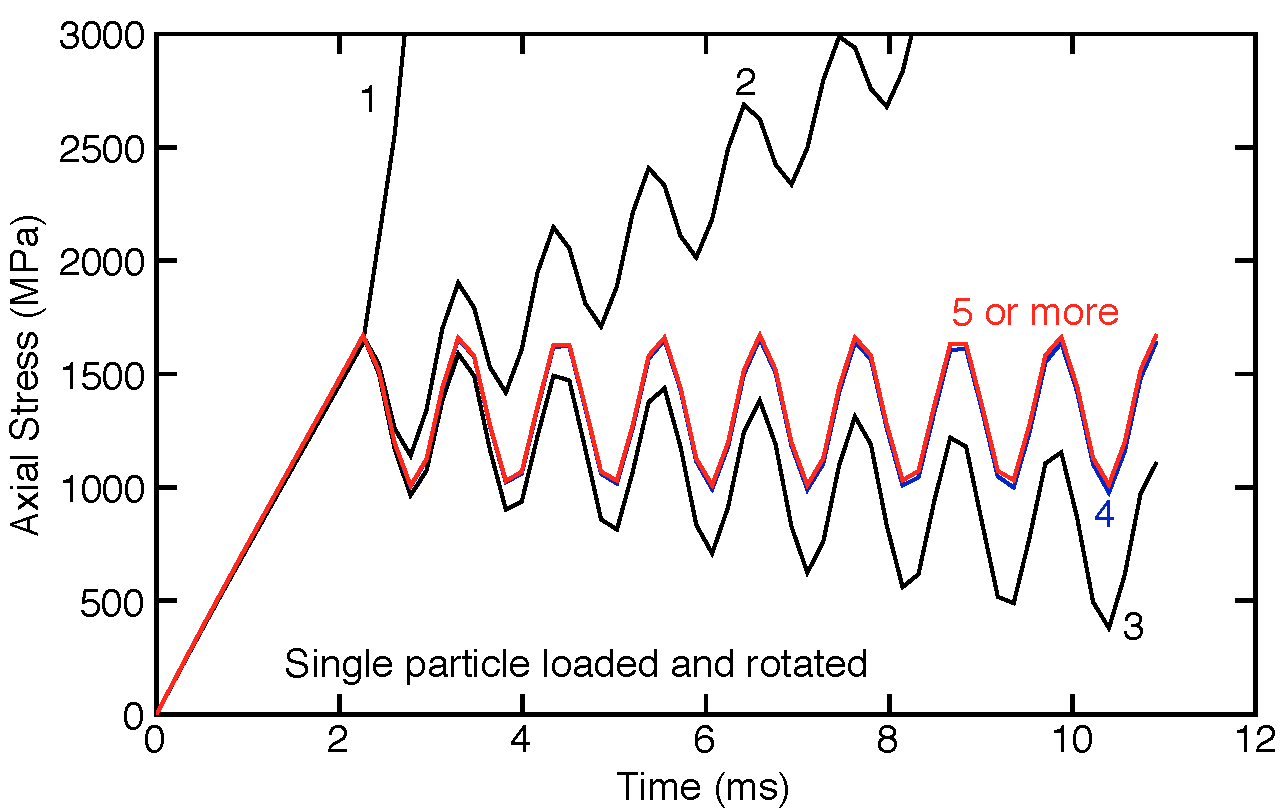
\includegraphics[width=5in]{IncrementalDef}
\caption{Calculation for a single particle loaded in tension, held, and then rotated. The different curves show $k_{max}$ or the number of terms used to expand the matrix exponential in the incremental deformation gradient.}
\label{dFCalc}
\end{center}
\end{figure}

\subsection{Mooney-Rivlin Material}

The Mooney-Rivilin material is an isotropic, elastic, hyperelastic material. It's stresses are based on a strain energy function that depends only on invariants to the left Cauchy-Green deformation tensor:
\begin{equation}
    \B = \F\F^T
\end{equation}
where $\F$ is the deformation tensor. The deformation tensor can be calculated by combining cumulative strain and rotation tensors (see {\tt HyperElastic.cpp} for the calculation). The strain energy is assumed to be
\begin{equation}
W = {G_1\over2}\left(\bar{I_1}-3\right) + {G_2\over2}\left(\bar{I_2}-3\right)^2 + {K\over2}\left(J-1\right)^2
\end{equation}
where $G_1$, $G_2$, and $K$ are material properties, $J=\det\F$, and the invariants are
\begin{eqnarray}
   \bar{I_1} & = & {B_{xx}+B_{yy}+B_{zz}\over J^{2/3}} \\
   \bar{I_2} & = & {1\over2}\left(\bar{I_1}^2 - {B_{xx}^2+B_{yy}^2+B_{zz}^2+2B_{xy}^2+2B_{xz}^2+2B_{yz}^2\over J^{5/3}}\right)
\end{eqnarray}
For low strains, this material is equivalent for a linear elastic, isotropic material with shear modulus $G_1+G_2$ and bulk modulus $K$. If $G_2=0$, the material is a neo-Hookean material. See below for an alternate compressibility terms. Some hyperelastic rubber models assume incompressible materials, which corresponds to $K\to\infty$; such models do not work in dynamic code (because wave speed is infinite).

The Cauchy (or true stress) is found by differentiating the strain energy to get
\begin{equation}
     \sigma = {G_1\over J^{5/3}}\left(\B - {I_1\over3}\I\right)
                     +  {G_2\over J^{7/3}}\left(I_1\B - \B^2 - {2I_2\over3}\I\right)   + K(J-1)\I
\end{equation}
where $I_1 = J^{2/3}\bar{I_1}$ and $I_2 = J^{4/3}\bar{I_2}$. The stress components can be divided into pressure, $P$, and deviatoric stress, $\vec s = \vec\sigma+P$, whichexplicitly evaluate to:
\begin{eqnarray}
      P & = & -K (J-1) \\
     s_{xx} & = & G_1{2B_{xx}-B_{yy}-B_{zz}\over 3J^{5/3}} + G_2{B_{xx}(B_{yy}+B_{zz})-2B_{yy}B_{zz}-B_{xy}^2-B_{xz}^2+2B_{yz}^2\over 3J^{7/3} }\\
      s_{yy} & = & G_1{2B_{yy}-B_{xx}-B_{zz}\over 3J^{5/3}}    + G_2{B_{yy}(B_{xx}+B_{zz})-2B_{xx}B_{zz}-B_{xy}^2+2B_{xz}^2-B_{yz}^2\over 3J^{7/3} }\\
      s_{zz} & = &  G_1{2B_{zz}-B_{xx}-B_{yy}\over 3J^{5/3}}    + G_2{B_{zz}(B_{xx}+B_{yy})-2B_{xx}B_{yy}+2B_{xy}^2-B_{xz}^2-B_{yz}^2\over 3J^{7/3} }\\
       s_{xy} & = &  G_1{B_{xy}\over J^{5/3}} + G_2{B_{zz}B_{xy}-B_{xz}B_{yz}\over J^{7/3}}\\
       s_{xz} & = & G_1{B_{xz}\over J^{5/3}} + G_2{B_{yy}B_{xz}-B_{xy}B_{yz}\over J^{7/3}}\\
       s_{yz} & = & G_1{B_{yz}\over J^{5/3}} + G_2{B_{xx}B_{yz}-B_{xy}B_{xz}\over J^{7/3}}
\end{eqnarray}

\subsubsection{Plane Strain and Plane Stress Analysis}

For 2D analysis, $F_{xz}=F_{yz}=F_{zx}=F_{zy}=0$, which leads to zero for corresponding terms in $\B$. The resulting stresses are $ P = -K (J-1)$ and
\begin{eqnarray}
      s_{xx} & = &  G_1{2B_{xx}-B_{yy}-B_{zz}\over 3J^{5/3}}  
                    + G_2{B_{xx}(B_{yy}+B_{zz})-2B_{yy}B_{zz}-B_{xy}^2\over 3J^{7/3} }\\
      s_{yy} & = &  G_1{2B_{yy}-B_{xx}-B_{zz}\over 3J^{5/3}}   
                     + G_2{B_{yy}(B_{xx}+B_{zz})-2B_{xx}B_{zz}-B_{xy}^2\over 3J^{7/3} }\\
      s_{zz} & = &   G_1{2B_{zz}-B_{xx}-B_{yy}\over 3J^{5/3}}   
                     + G_2{B_{zz}(B_{xx}+B_{yy})-2B_{xx}B_{yy}+2B_{xy}^2\over 3J^{7/3} }\\
       s_{xy} & = &  G_1{B_{xy}\over J^{5/3}} + G_2{B_{zz}B_{xy}\over J^{7/3}}\\
       s_{xz} & = & 0 \\
       s_{yz} & = & 0
\end{eqnarray}
For plane strain analysis $B_{zz}=1$. For plane stress analysis, one has to solve numerically for $B_{zz}$ to get $\s{zz}=0$ or $s_{zz}=P$ and then use that result to find $\e{zz}$ and other stresses.

\subsubsection{Dealing with Thermal and Moisture Strains}

To handle thermal and moisture strains the deformation is divided into two steps. The first is free expansion to the new stress free volume and then deformation to the final volume. The total deformation will be
\begin{equation}
      \F = \F^* \F^{res} = \F^* \lambda_{res}\tens I
\end{equation}
where $\lambda_{res}$ is total extension due to free thermal and moisture expansion:
\begin{equation}
    1 + \alpha\Delta T + \beta \Delta c
\end{equation}
The stresses and energy, however, should be found using $\F^*$ instead of $\F$, where $\F^*$ is now deformation from the current free expansion volume instead of from the initial volume. The net effects are $\F^* = \F/\lambda_{res}$, $J_{eff} = |\F^*| = J/\lambda_{res}^3$, and $\B_{eff} = \B/\lambda_{res}^2$.

When doing incremental deformation, $\F_{k+1} = \tens{dF}\thinspace\F_k$ and incremental volume ratio is $dJ = |\tens{dF}| = V_{k+1}/ V_k$, but $J_{eff}$ is $V/V_{sf}$ where $V_{sf}$ is the current stress free volume. For incremental deformation, $J_{k+1} = dJ J_k$, but we really want to increment $J_{eff,k+1} = dJ_{eff}J_{eff,k}$, which is\begin{equation}
     J_{eff,k+1} = {V_{k+1}\over V_{sf,k+1}} = {V_{k+1}\over V_{k}}{V_{sf,k}\over V_{sf,k+1}} {V_{k}\over V_{sf,k}}
             = {V_{k+1}\over V_{k}}{V_{sf,k}\over V_{sf,k+1}} J_{eff,k} = dJ_{eff}J_{eff,k}
\end{equation}
which implies that
\begin{equation}
      dJ_{eff} = {V_{k+1}\over V_{k}}{V_{sf,k}\over V_{sf,k+1}} = dJ/d\lambda_{res}^3
\end{equation}
where
\begin{equation}
    d\lambda_{res} = 1 + \alpha dT + \beta dc
\end{equation}
where $dT$ and $dc$ are temperature and concentration changes on the current time step.

\subsubsection{Alternate Bulk Modulus Term}

Two alternative compressibility terms (showing only that term) is

\begin{equation}
W = {K\over2}(\ln J)^2  \qquad{\rm and}\qquad W = {K\over2}\left({1\over2}(J^2-1) - \ln J\right)
\end{equation}

\noindent which gives normal Cauchy pressure terms of
\begin{equation}
     P = -K {\ln J\over J}\I  \qquad{\rm and}\qquad P = - {K\over 2}\left(J-{1\over J}\right)\I
\end{equation}

\noindent Although these three compressibility terms show some significant differences when $J$ deviates significantly from 1, under most problems, $J$ will stay close to one. Two exceptions could be constrained compression or tension. Here, the only one that works well to very small or large $J$ is the second one above. This one correctly leads to inifinite positive stress as $J\to\infty$ and infinite negative stress as $J\to0$. This later one is the default for this material in {\tt NairnMPM}.

\subsubsection{Tangent Bulk Modulus}

The incremental bulk modulus is
\begin{equation}
   {1\over K(P)} = - {d\ln V\over dP} = - {d\ln J\over dP}  \qquad{\rm or} \qquad K = -J {dP\over dJ}
\end{equation}
The various bulk moduli are
\begin{eqnarray}
   P = -K_0(J-1) &\qquad{\rm gives}\qquad & K = K_0 J \\
   P = -K_0 {\ln J\over J} &\qquad{\rm gives}\qquad& K_0{1-\ln J\over J^2}\\
   P = - {K_0\over 2}\left(J-{1\over J}\right) &\qquad{\rm gives}\qquad& K = {K_0\over 2}\left(J + {1\over J}\right)
\end{eqnarray}



\subsection{Mie-Gr\"{u}niesen Equation of State}

The Mie-Gr\"{u}niesen Equation of State defines the pressure only and the Kirchoff pressure needed in {\tt NairnMPM} is
\begin{equation}
       P = {C_0^2 \eta \left(1 - {1\over 2}\gamma_0 \eta\right) \over (1 - S_1\eta - S_2\eta^2 - S_3 \eta^3)^2} + \gamma_0 U
\end{equation}
where $\eta$ is fraction compression and given by
\begin{equation}
    \eta = 1 - {\rho_0\over \rho} = 1 - {V\over V_0} = 1 - J
\end{equation}
and $\gamma_0$, $C_0$, and $S_i$ are material properties and $U$ is total internal energy. The above equation applies only in compression ($\eta>0$). In tension, the pressure is given by
\begin{equation}
      P = C_0^2\eta + \gamma_0 U
\end{equation}

This equation of state also causes a temperature change of
\begin{equation}
     dT = - T \gamma_0 {\rho_0\over \rho} {V(t+\Delta t)-V(t)\over V} + {dq \over C_V}
\end{equation}
where $dq$ is dissipated energy that is converted to heat. The first term simplifies to an isentropic temperature change of
\begin{equation}
     dT_{dq=0} = - JT \gamma_0  {V(t+\Delta t)-V(t)\over V} 
\end{equation}
The volume change relative to current volume can be found from
\begin{equation}
     {V(t+\Delta t)-V(t)\over V(t+\Delta t)} =1 - {1\over |dF|}
\end{equation}

Noticing that
\begin{equation}
     {dT_{dq=0}\over T} =   \gamma_0  d\eta
\end{equation}
The temperature due to isoentropic heating alone can be integrated to
\begin{equation}
     T = T_0\exp( \gamma_0  \eta)
\end{equation}
Thus the total temperature rise (assuming $C_V$ is constant) is
\begin{equation}
      dT = T_0(\exp( \gamma_0  \eta)-1)\bigr) + {\Phi\over C_V}
\end{equation}
where $\Phi$ is the cumulative dissipated energy due to plasticity.

Rather then calculate temperature changes, which are needed for internal energy, {\tt NairnMPM} tracks total work, $w$, and heat, $q$, to find internal energy as $U = w+q$. The details are given above in the section on ``Thermodynamics of Deformation.''

In compression, $J$ is physically limited to be between 0 and 1, which means $\eta$ is also between 0 and 1. But for most materials that have been fit to this equation of state, the denominator in pressure will be come zero before $eta$ reaches 1. For example, Tungsten has $S_1=1.24$ and $S_2=S_3=0$. The denominator becomes zero when
\begin{equation}
     \eta = 1/1.24 = 0.806
\end{equation}
If the time step is too large in dynamic code, the compression could potentially pass this value. If that happens for any particle, the results will likely be poor; {\tt NairnMPM} prints a warning labeling states beyond the physical limit as ``excessive compression.'' It is good practice to use an adjustable time step when using this material so the time step can get smaller if the compression gets high.

This equation of state has no thermal expansion coefficient, but thermal expansion occurs naturally with proper tracking of heat flow and temperature. The volumetric thermal expansion coefficient from input properties is:
\begin{equation}
     3\alpha = {\rho_0 \gamma_0 C_V\over K_0} \qquad{\rm or}\qquad \gamma_0 = {3K_0\alpha\over \rho_0 C_V}
\end{equation}
which is same as defined above in Eq.~(\ref{gamzdef}). The temperature rise here, which is
\begin{equation}
     dT_{dq=0} = - J T\gamma_0 {\Delta V\over V}    \quad vs. \qquad  dT_{dq=0} -JT_0  {K\over K_0} \gamma_0 {\Delta V\over V}     \label{mgdt}
\end{equation}
from above. The result here differs by a factor $(T/T_0)(K/K_0)$.

\subsection{Ideal Gas Law}

The ideal gas material implements ideal gas law as a large deformation, hyperelastic material. It seems to work well for gas confined within a solid or constrained by rigid particles. It does not handle gas dynamics such as irreversible free expansion, but does handle reversible processes including coupled conversion of energy into heat ({\em i.e.}, cooling on expansion and heating on compression).

The ideal gas law is
\begin{equation}
    PV = nRT
\end{equation}
The ideal gas properties are defined by picking any reference pressure, $P_0$, reference temperature, $T_0$, and reference density, $\rho_0$. If $M$ is the molecular weight of the gas molecules, the reference density can be found from:
\begin{equation}
    \rho_0 = {P_0\over T_0} {M\over R}
\end{equation}
We can now eliminate $n$ and $R$ to derive
\begin{equation}
    P = P_0{V_0\over V}{T\over T_0} = P_0 {T\over T_0} {1\over J} \label{geniglaw}
\end{equation}
where $J = \det \F = V/V_0$. The Cauchy stress due to this pressure is $-P\I$, which implies hyperelastic energy function determined from:
\begin{equation}
    \vec\sigma = - P_0 {T\over T_0} {1\over J}\I = {dU(J)\over dJ}\I
        \qquad{\rm or}\qquad
         U(J) = - P_i \ln J
\end{equation}
where $P_i = P_0T/T_0$ is the initial pressure (when $J=1$). This energy is equal to the energy per unit initial volume for isothermal compression or expansion of an ideal gas:
\begin{equation}
    U(J) = - {1\over V_0} \int_{V_0}^V P\thinspace dV = - {P_0T\over T_0} \int_{V_0}^V {1\over V}\thinspace dV = - P_i \ln {V\over V_0} = - P_i \ln J
\end{equation}

For MPM calculations, the code needs a specific Kirchoff stress normalized to $\rho_0$ or
\begin{equation}
    \vec\tau^{(s)} = -{PJ\over \rho_0}\I  = - {P_0\over \rho_0} {T\over T_0}\I
\end{equation}
In coding, an incremental approach is preferred. 
If $\tau_n^{(s)}$ is any diagonal element of the specific Kirchoff stress tensor for time step $n$, then
\begin{equation}
   \tau_{n+1}^{(s)} = - {P_0\over \rho_0} {T_{n+1}\over T_0}  = - {P_0\over \rho_0} {T_n\over T_0} {T_{n+1}\over T_n}
       = \tau_n^{(s)} {T_{n+1}\over T_n}
\end{equation}
Note that the Kirchoff stress remains constant for isothermal expansion and compression.

The energy increment associated with this stress change is $dU = -P\thinspace dV$ work. The energy per unit mass using midpoint rule between initial and final pressure is therefore
\begin{equation}
    {dU\over \rho_0 V_0} = - {1\over2} {P_n+P_{n+1}\over \rho_0} 
         {V_{n+1} - V_n\over V_0} = - {1\over2} {P_n+P_{n+1}\over \rho_0} {V_{n+1}\over V_0}
         \left(1 - {V_n\over V_{n+1}}\right)
\end{equation}
Let deformation gradient for step $n+1$ be
\begin{equation}
       \F_{n+1} = \f\cdot\F_n  \quad{\rm where}\quad \f = \exp(\Delta t\nabla\vec v)
       \quad{\rm and}\quad J_{n+1} = \det \f \thinspace J_n
\end{equation}
which leads to
\begin{equation}
    {dU\over \rho_0 V_0} = - {J_{n+1}\over2} {P_n+P_{n+1}\over \rho_0} 
         \left(1 - {1\over\det f}\right) = - {1\over2}
         \left({P_n\over \rho_{n}}\det f+{P_{n+1}\over \rho_{n+1}} \right)
         \left(1 - {1\over\det f}\right)
\end{equation}
But, $P/\rho$ is $-\tau^{(s)}$ leading to
\begin{equation}
    {dU\over \rho_0 V_0} =  {1\over2}
         \left(\tau_n^{(s)}\det f+\tau_{n+1}^{(s)} \right)
         \left(1 - {1\over\det f}\right)
\end{equation}

In {\tt NairnMPM}, the cumulative work, $w$, is tracked in the particle's strain energy and cumulative heat, $q$, in the heat energy (heat energy will be zero for adiabatic or $-w$  for isothermal). The internal energy is $U = w + q$. The incremental work is $dw = dU/(\rho_0 V_0)$ term above. Because plastic energy has no other use, it is used in this material to track the change in entropy using
\begin{equation}
      dS =\left\{ \begin{array}{ll}
                d_iS + {C_V dT\over T} - {C_V dT_{ad}\over T + dT_{ad}} & {\rm locally\ adiabatic} \\
                d_iS + {C_V dT-d\Phi\over T} & {\rm locally\ isothermal}
                \end{array} \right. \\
\end{equation}
where $dT_{ad} = dU/C_V$ is the temperature rise that would occur if the process was adiabatic and the irreversible entropy, $d_iS$, is assumed to be zero. The reason that $dS\ne0$ for adiabatic case is because there might be temperature changes due to external conditions or conduction. The Helmholtz free energy can be found post analysis using $A = U - TS = w + q - TS$.

When gas particles are present, they have to be initialized to the pressure (or stress) of
\begin{equation}
     \tau_i^{(s)} =  - {P_i\over \rho_0} = - {P_0\over \rho_0} {T\over T_0}
\end{equation}
where $T$ is the simulation reference temperature (need not be the gas reference temperature, which can be any desired reference condition). All simulations with gas particles must therefore specify a reference temperature in degrees Kelvin.

This material always needs heat capacity and needs thermal conductivity when doing conduction. Heat capacity is calculated using ideal gas law theory ($C_V=(3/2)nR/(\rho_0 V_0)$ for monotonic gas and $C_V=(5/2)nR/(\rho_0 V_0)$ for diatomic gas in J/(kg-K)). To find heat capacity from input parameters, substitute $nR = P_0V_0/T_0$ at reference conditions to get
\begin{equation}
     C_V =  {3\over 2} {P_0 \over \rho_0T_0}
\end{equation}
for monatomic gas (or replace $3/2$ with $5/2$ for diatomic gas). For conduction, the current code assumes conductivity is a temperature-independent property (as entered), although conductivity of a gas does vary with temperature. If simulations with large temperature changes of the gas are important, this material will need to be improved to allow temperature-dependent thermal conductivity.

For wave speed calculations, the bulk modulus for adiabatic conditions is
\begin{equation}
   B = \sqrt{\gamma\rho R T\over M}
\end{equation}
In terms of defined material properties, the wave speed reduces to
\begin{equation}
   C = \sqrt{B\over\rho} = \sqrt{{5\rho_0P_0T\over 3T_0}}
\end{equation}
where $T$ is particle temperature.


\subsection{Verification Examples}

A simple gas problem is to confine all sides by rigid particles and move one wall for compression or expansion. If the movable wall is in the $x$ direction, the volume will be $V = V_0(1+\e{xx})$. For isothermal compression and expansion:
\begin{eqnarray}
    P & = & {P_i\over 1+\e{xx}} \\
    U & = & 0 \\
    w & = & -P_iV_0\ln(1+\e{xx}) \\
    q & = & -w \\
    S & = & nR\ln(1+\e{xx}) = {P_0 V_0\over T_0}\ln(1+\e{xx})
\end{eqnarray}
For adiabatic compression and expansion
\begin{eqnarray}
    P & = & {P_i\over (1+\e{xx})^\gamma} \\
    T & = & {T_i\over (1+\e{xx})^{\gamma-1}} \\
    U & = & C_V(T - T_i) 
               = {3P_0V_0\over 2T_0}T_i\left({1\over (1+\e{xx})^{\gamma-1}}-1\right) \\
    w & = & U \\
    q & = & 0 \\
    S & = & -(\gamma-1)C_V\ln(1+\e{xx}) + {P_0 V_0\over T_0}\ln(1+\e{xx}) = 0
\end{eqnarray}
where $\gamma=C_P/C_V=5/3$. An undocumented custom task in {\tt NairnMPM} can subject an ideal gas to a Carnot cycle and recover an efficiency close to the theoretical maximum of:
\begin{equation}
       \eta = 1 - {T_2\over T_1}
\end{equation}
where $T_1$ is the hot reservoir and $T_2$ is the cold one.

\subsection{Isothermal {\em vs.} Adiabatic {\em vs.} General Constitutive Law}

Equation (\ref{geniglaw}) can be rewritten as an increment in pressure from initial pressure $P_0$ at temperature $T_0$:
\begin{equation}
    P - P_0 = \kappa_0\left[\left(J_{res}\over J\right)-1\right]
\end{equation}
where $\kappa_0$ is the bulk modulus at $P_0$:
\begin{equation}
   {1\over \kappa_0} = -{1\over V_0} \left({\partial V_0\over \partial P}\right)_T = {1\over P_0}
\end{equation}
and
\begin{equation}
    J = {V(P,T)\over V(P_0,T_0)}={V\over V_0} \qquad{\rm and}\qquad J_{res} = {V(P_0,T)\over V(P_0.T_0)} = {T\over T_0}
\end{equation}
Here $J_{res}$ is the volume ratio for free thermal expansion at reference pressure $P_0$. For an isothermal process $J_{res}=1$. For a (reversible) adiabatic compression or expansion, the temperature change is:
\begin{equation}
       T = {T_0\over J^{\gamma-1}} \qquad{\rm and}\qquad J_{res} = {1\over J^{\gamma-1}}
\end{equation}
Two special cases of the general law, therefore, are:
\begin{eqnarray}
   P - P_0 & = & \kappa_0\left[\left(1\over J\right)-1\right]  \qquad{\rm isothermal} \\
   P - P_0 & = & \kappa_0\left[\left(1\over J\right)^\gamma-1\right]  \qquad{\rm adiabatic}
\end{eqnarray}
But if code implements either of these laws, it will be restricted to either isothermal or adiabatic conditions only. The preferred approach is to implement the general law because it includes both these limits as special cases and can be used for nonisothermal, nonadiabatic simulations as well. When using a general law, however, each  material point must correctly change its temperature according to how much energy should be converted into heat for a given increment in deformation. For an ideal case undergoing in increment in volume of $dV$, the temperature change is
\begin{equation}
    dT = -{P dV\over C_V} = -{nRT \over C_V}{dV \over V} = -{nRT \over C_V}{\rho\over\rho_0}{dV \over V_0}
\end{equation}
In other words, all the work is converted into heat. Also notice that this result can be written
\begin{equation}
    {dT\over T} = {nR \over C_V}{1\over J}d\eta = {\gamma_0\over J}d\eta = -\gamma_0{dJ\over J} \qquad{\rm where}\qquad \eta = 1 - {\rho_0\over \rho} = 1 - J
\end{equation}
For a monatoic ideal gas $\gamma_0=2/3$; for a diatomic gas $\gamma_0=2/5$; for both $\gamma_0=\gamma-1$. This result is identical to the Mie-Gr\"{u}niesen theory in Eq.~(\ref{mgdt}) by using $K=P$, $3\alpha=1/T$ and $C_V = (3/2)nR/(\rho V)$ (or 5/2 for diatomic gas).

\subsection{Van der Waals Gas Law}

The van der Wasls gas material implements a non-ideal gas law as a large deformation, hyperelastic material. It seems to work well for gas confined within a solid or constrained by rigid particles. It does not handle gas dynamics such as irreversible free expansion, but does handle reversible processes including coupled conversion of energy into heat ({\em i.e.}, cooling on expansion and heating on compression).

The van der Wasls gas law is
\begin{equation}
    \left(P-{an^2\over V^2}\right)\left({V\over n}-b\right) = RT
\end{equation}
The nonideal gas properties are defined by picking any reference pressure, $P_0$, reference temperature, $T_0$, and reference density, $\rho_0$, along with $a$ and $b$. The law can then be transformed to
pressure of
\begin{equation}
    P = \left(P_0-a'\right)\left(1-b'\over J-b'\right){T\over T_0} + {a'\over J^2}
\end{equation}
where $J = V/V_0$, $V_0$ is initial particle volume, $a'=an^2/V_0^2$, and $b'=nbV_0$. Writing $P = - dU(J)/dJ$ implies a hyperelastic energy function of
\begin{equation}
    U(J) = \left(P_i-a'\right)\left(1-b'\right)\ln (J-b') - {a'\over J}
\end{equation}
where $P_i$ is the initial particle pressure (when $J=1$) of
\begin{equation}
    P_i = \left(P_0-a'\right){T\over T_0} + {a'}
\end{equation}
This energy is equal to the energy per unit initial volume for isothermal compression or expansion of an ideal gas:
\begin{equation}
    U(J) = - {1\over V_0} \int_{V_0}^V P\thinspace dV = -  \int_{1}^J \left(\left(P_i-a'\right)\left(1-b'\over J-b'\right) + {a'\over J^2}\right)\thinspace dJ
    \end{equation}

In {\tt NairnMPM}, the cumulative work is tracked in the particle's plastic energy (which is $=PdV$ work and can tracked the same as for an ideal gas). The particle's strain energy tracks total internal energy in the gas per unit mass, which for a van der Waals gas is
\begin{equation}
   U = C_V(T-T_0) - {a'\over  \rho_0 J}
\end{equation}
In hyperelastic code, an incremental form is
\begin{equation}
   U = C_V dT + {a'\over \rho_0 J^2} dJ
\end{equation}

For a van der Waals gas, the heat capacity is same as for ideal gas, $C_V=(3/2)nR/(\rho_0 V_0)$ for monatomic (or 5/2 for diatomic gas), the the $n$ is found differently from reference conditions. It can be found as root to
\begin{equation}
     {ab\over V_0^2} n^3 - {a\over V_0} n^2 - (P_0b+RT_0)n + P_0V_0 = 0
\end{equation}
This $n$ is needed to find $a'$, $'b'$ and $C_V$.


\section{Two-State Isotropic Material}

The \code{BistableIsotropic} class inherits from \code{Isotropic}. It allows two different isotropic states and transitions  between the states based on various criteria. The two options are to have a jump to a new linear stress-strain curve (\code{DILATION\_RULE}) or to simply change the slope (\code{DISTORTION\_RULE} or \code{VONMISES\_RULE}). When jumping to a new curve (\code{DILATION\_RULE}), the deformed state can additionally define a new origin by adding an offset volumetric strain. The only new calculations needed are to change properties when a transition occurs and if there is a new stress-strain curve to calculate a jump in stresses to the new curve. The 3D stiffness equations with an offset volumetric strain for an isotropic material are
\begin{equation}
     \left(\begin{array}{c} \s{xx} \\ \s{yy} \\ \s{zz} \\ \t{xz} \\ \t{yz} \\ \t{xy} \end{array}\right)
       =  \left(\begin{array}{cccccc}
      C_{11} & C_{12} & C_{12} & 0 & 0 & 0 \\
      C_{12} & C_{11} & C_{12} & 0 & 0 & 0 \\
      C_{12} & C_{12} & C_{11} & 0 & 0 & 0 \\
      0 & 0 & 0 & C_{66} & 0 & 0 \\
      0 & 0 & 0 & 0 & C_{66} & 0  \\
      0 & 0 & 0 & 0 & 0 &  C_{66}  \end{array}\right)
     \left(\begin{array}{c} \e{xx} - {\Delta\over 3} -\er{}\\ \e{yy} - {\Delta\over 3} -\er{}\\ 
                   \e{zz} - {\Delta\over 3} - \er{}\\ 
                   \g{xz} \\ \g{yz} \\ \g{xy} \end{array}\right)
\end{equation}
where $\er{}=\a{}\DT+\b{}\Delta c$.
Whenever a change in state occurs in the \code{DILATION\_RULE}, these equations must be used to recalculate all components of stress.

\subsection{Plane Stress Equations}

The plane stress stiffness equations for in-plane stresses are
\begin{equation}
      \vvec{\s{xx}}{\s{yy}}{\t{xy}} = \symmat{Q_{xx}}{Q_{xy}}{0}{Q_{xx}}{0}{Q_{xyxy}}
          \vvec{\e{xx}- {\Delta\over 3}  - \er{}}{\e{yy}- {\Delta\over 3}  - \er{}}{\g{xx}}
 \end{equation}
with out-of-plane strain given  by
\begin{equation}
            \e{zz} = -{C_{12}\over C_{11}}(\e{xx}- {\Delta\over 3} -\er{}) - {C_{12}\over C_{11}}(\e{yy} - {\Delta\over 3}-\er{}) 
                   + {\Delta\over 3}  + \er{}
\end{equation}
For the super-class \code{Isotropic} material, the needed terms are stored as \code{C[1][1]} = \code{C[2][2]} $= Q_{xx}/\rho$,  \code{C[1][2]} $= Q_{xy}/\rho$,  \code{C[3][3]} $= Q_{xyxy}/\rho$,  \code{C[4][1]} =  \code{C[4][2]}$= -C_{12}/C_{11}$,  \code{alpha[1]} = \code{alpha[2]} = \code{alpha[4]} = \code{CTE3}  $=\a{}$, \code{beta[1]} = \code{beta[2]} = \code{beta[4]} = \code{CME3}  $=\b{}$, \code{C[1][3]} = \code{C[2][3]} = \code{alpha[3]} =\code{beta[3]} $=0$, and \code{normOffset} $=\Delta/3$.

\subsection{Plane Strain Equations}

The plane strain stiffness equations for in-plane stresses are
\begin{equation}
      \vvec{\s{xx}}{\s{yy}}{\t{xy}} = \symmat{C_{11}}{C_{12}}{0}{C_{11}}{0}{C_{66}}
          \vvec{\e{xx} - {\Delta\over 3}(1+\nu) - \err{}}{\e{yy} - {\Delta\over 3}(1+\nu)  - \err{}}{\g{xx}}
 \end{equation}
 where $\err{}=\a{}^{(r)}\DT+\b{}^{(r)}\Delta c$.
 In other words, a reduced offset and residual strains are needed. The out-of-plane stress is found from 3D equation and without reduced terms:
 \begin{equation}
            \s{zz} = C_{12}\left(\e{xx} - {\Delta\over 3} -\er{}\right) 
                            +C_{12}\left(\e{yy} - {\Delta\over 3} -\er{}\DT\right) 
                            -C_{11}\left({\Delta\over 3} +\er{}\right) 
\end{equation}
For the super-class \code{Isotropic} material, the needed terms are stored as \code{C[1][1]} = \code{C[2][2]} = \code{C[4][4]} $= C_{11}/\rho$,  \code{C[1][2]} $= C_{12}/\rho$,  \code{C[3][3]} $= C_{66}/\rho$,  \code{C[4][1]} =  \code{C[4][2]} $= C_{12}/\rho$, \code{alpha[1]} = \code{alpha[2]} $=\a{}(1+\v{})$, \code{beta[1]} = \code{beta[2]} $=\b{}(1+\v{})$, \code{alpha[4]} = \code{CTE3} $=\a{}$, \code{beta[4]} = \code{CME3} $=\b{}$, \code{alpha[5]} = \code{alpha[6]} $=\nu$, \code{C[1][3]} = \code{C[2][3]} = \code{C[4][3]} = \code{alpha[3]} = \code{alpha[7]} $=0$, \code{normOffset} $=\Delta/3$, and \code{nu} = $\v{}$.

\subsection{Special Cases for $E=0$}

If either $K$ or $G$ in any state is zero then the tensile modulus $E$ is also zero. Although this state is easy to derive in theory, in practice, it rarely gives useful results in dynamic MPM (except maybe as an inclusion in a composite material). A second problem is that it requires special cases to make it work with the super \code{Isotropic} class because that class has equations requiring $E\ne 0$. For these reasons, NairnMPM does not support zero modulus states in this material. It is easy to approximate such a state simply by setting $K$ and/or $G$ to a very small number.

\end{document}   